% !TeX program  = XeLaTeX
% !TeX encoding = UTF-8

\documentclass[UTF8]{ctexart}

\usepackage[
    colorlinks=true,
    linkcolor=black,
    urlcolor=black,
    bookmarksopen=true
    pdfauthor={蒋翌坤},
    ]{hyperref}
\usepackage{bookmark}
\usepackage[export]{adjustbox}
\usepackage{amsmath}
\usepackage{pgfplotstable}
\usepackage{booktabs}
\usepackage{tabularx}
\usepackage{indentfirst}
\usepackage[inline]{enumitem}
\usepackage[inkscapeversion=1.2.2]{svg}
\usepackage{caption}
\usepackage{subcaption}
\usepackage{makecell}
%\usepackage{chngcntr}
%\counterwithin{figure}{section}
%\counterwithin{table}{section}

\usepackage{template}

\newcommand{\hmwkTitle}{疫情下的谣言传播可视分析系统}
\newcommand{\hmwkClass}{程序设计与数据可视化}

\newcommand{\figwidth}{0.8\linewidth}


\begin{document}

\clearpage
\makecover

\pagebreak

\tableofcontents

\pagebreak
\pagenumbering{arabic}

\section{数据预处理}
本次研究的数据集为~\verb|rumor.csv|,其中包含了366条谣言数据。鉴于数据背景、来源、变量含义以及预期目标已经在作业中给出,此处不再赘述。
在数据处理、分析前,我们将数据存储在~\verb|pandas.DataFrame|~类中,以便于后续的数据处理与可视化分析。

\subsection{数据预处理步骤}

在此节中,我们将对数据集进行预处理,为接下来的数据可视化分析打下基础。
首先,选取数据集的前5条谣言数据,观察数据集的部分内容及描述性统计,确定预处理数据的步骤。
数据集前5条谣言数据如表~\ref{tab:datasetContent}~所示。
数据集各变量在~\verb|DataFrame|~中的类型及部分描述性统计如表~\ref{tab:datasetVariable}~所示。

\begin{table}[!ht] \centering
    \begin{tabularx}{\linewidth}{X c c c c c c c}
        \toprule
        date & source & content & province & user\_0 & \dots & user\_17 & like \\
        \midrule
        2022-02-18 & 北京日报客户端 & 有人从香港\dots & 广东 & 0 & \dots & 0 & 0 \\
        2022-02-18 & 大河报、羊城晚报 & 近日,社交\dots & 河南 & 0 & \dots & 0 & 41 \\
        2022-02-17 & 南方都市报、大众网 & 近日,网传\dots & 湖南 & 0 & \dots & 0 & 26 \\
        2022-02-17 & 江苏省互联网举报中心 & 近日,网传\dots & 江苏 & 0 & \dots & 0 & 31 \\
        2022-02-16 & 中国新闻网 & 在塞企业机\dots & \color{red}{NaN} & 0 & \dots & 0 & 0 \\
        \bottomrule
    \end{tabularx}
    \caption{数据集前5条谣言数据}
    \label{tab:datasetContent}
\end{table}

\begin{table}[!ht] \centering
    \begin{tabularx}{\linewidth}{X c c c c c c c c}
        \toprule
        变量名 & date & source & content & province & user\_0 & \dots & user\_17 & like \\
        \midrule
        类型 & object & object & object & object & int64 & \dots & int64 & int64 \\
        非空值 & 366 & 360 & 366 & 277 & 366 & \dots & 366 & 366 \\
        均值 & - & - & - & - & 0.19 & \dots & 0.02 & 72.59 \\
        最小值 & - & - & - & - & 0 & \dots & 0 & 0 \\
        中位数 & - & - & - & - & 0 & \dots & 0 & 34 \\
        最大值 & - & - & - & - & 1 & \dots & 1 & 2495 \\
        \bottomrule
    \end{tabularx}
    \caption{数据集变量类型及部分描述性统计}
    \label{tab:datasetVariable}
\end{table}

分析表~\ref{tab:datasetContent}~和表~\ref{tab:datasetVariable}~内容,可以发现以下几个问题
\footnote{注意到数据集中user\_0到user\_17变量应该为Bool类型变量,但目前是int64类型的0-1变量,不妨碍分析。}:
% NOTE: 这一点不是很确定要不要写
\begin{enumerate}
    \item 数据集中source、province变量存在NaN值,需要对这些缺失值进行处理;
    \item 数据集中date变量应该为Datetime类型,但目前是object类型,需要进行类型转换才能进行与时间相关的分析;
    \item 数据集中like变量最小值、最大值差距很大,而中位数远小于均值,说明like变量的分布严重左偏。
\end{enumerate}

根据上述通过观察得到的问题,我们的预处理分为以下几个步骤\footnote{由于数据集中的每条谣言数据主要由谣言文本构成,因此不涉及离群值处理}:
\begin{enumerate}
    \item 数据缺失值处理。对于source、province变量的缺失值,
    由于谣言来源或涉及省份和谣言内容紧密相关,可以通过观察谣言内容结合搜索引擎,手动将这些缺失值填上;
    对于那些无法分辨出谣言来源或涉及省份时,填充数据或删除该条谣言数据都不合理,因此保留NaN值,
    在后续涉及source或province的分析过程中,忽略这些缺失值对应的谣言数据。
    \item 数据重复值处理。由于重复值的出现可能会影响分析结果,而数据集中谣言数量较小,可以通过观察法来判断数据集中是否存在重复值。
    % 如果存在重复值,则以谣言发布时间最早的为准。
    % NOTE: 如果有重复值,要写处理的方法
    \item 数据类型转换。将数据集中的date变量转换为Datetime类型。 % NOTE: user\_0到user\_17变量可能会改
    \item 变量数值变换。like变量与对like变量每个值取$\ln(x+1)$如图~\ref{fig:like_loglike_hist}~所示,
    从图中可以发现对like变量每个值取$\ln(x+1)$能更加接近正态,因此,可以对like变量每个值取$\ln(x+1)$并保存在新的变量log\_like中。
    \item 分词处理。将数据集中的content变量通过~\verb|jieba|~库进行分词处理。
    在分词时,利用自定义停用词表\footnote{见附录~\ref{subsec:stopwords}~}中的词作为停用词,不进行分词。
    分词后的结果(一个list)保存在新的变量content\_token中。 % NOTE: 可能source\_token没必要
\end{enumerate}

\begin{figure}[!ht]
    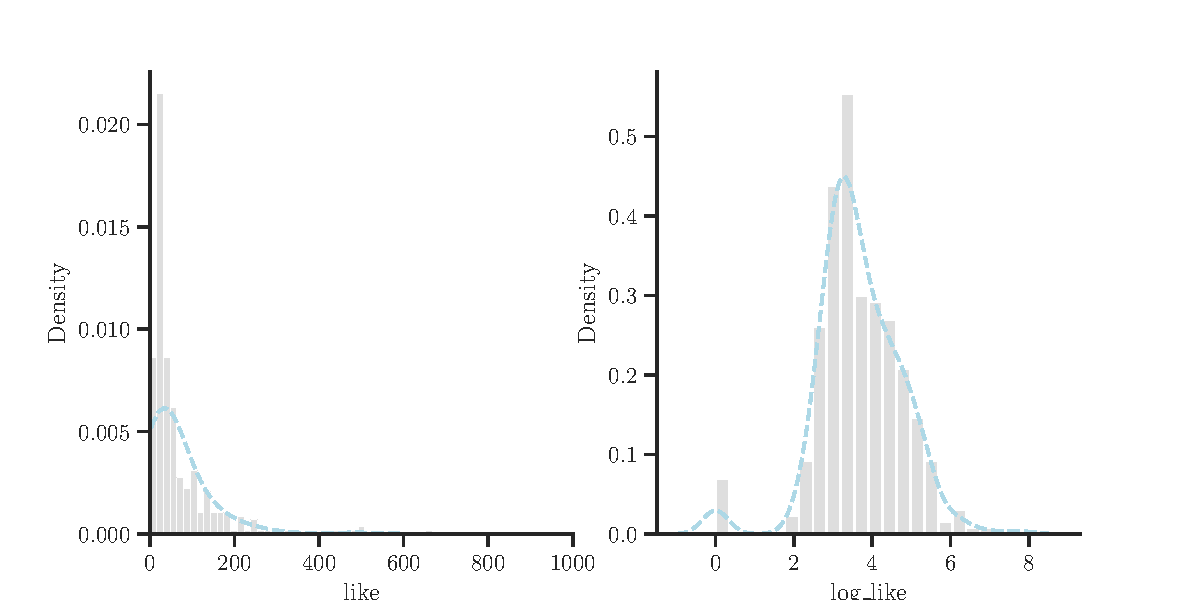
\includegraphics[width=\linewidth]{../figures/loglike_like_hist}
    \caption{like变量与log\_like变量的直方图}
    \label{fig:like_loglike_hist}
\end{figure}

\subsection{数据预处理结果}

根据上节提到的预处理步骤,我们对数据集进行了预处理。在数据预处理时,得到了以下结果:
\begin{enumerate}
    \item 由于谣言来源难以查找,填充了0个source变量缺失值;填充了32个province变量缺失值,这一变量的缺失值填充较为容易:
    例如第7条谣言数据的province变量为缺失值,谣言信息为“网传横州市马山镇太宁村有一阳性病例接触者?谣言!”,
    根据“横州市马山镇”的地理信息,可以判断该谣言涉及广西省,
    因此将原本的缺失值填充为“广西”。
    \item 数据集中不存在重复值。
    \item ~\verb|jieba|~库在处理地名时有分词问题,再以第7条谣言数据举例,分词结果为:[网传, 横, 州市, 马, 山镇, 太宁, 村有, 阳性, 病例, 接触, 谣言],
    但“横州市”、“太宁村”应该作为一个词。因此,我们需要对分词结果进行处理,纠正这一地名问题。
    但是具体地名在之后的分析过程不重要,对分析结果的影响不大,而处理地名问题十分复杂,收益远大于付出,因此我们不再对分词结果进行处理。
\end{enumerate}

预处理后的数据集部分内容如表~\ref{tab:datasetPreprocessedVariable}~所示。

\begin{table}[!ht] \centering
    \begin{tabularx}{\linewidth}{X c c c c c c c}
        \toprule
        变量名 & date & source & content & province & \dots & log\_like & content\_token \\
        \midrule
        类型 & datetime64[ns] & object & object & object & \dots & float64 & object \\
        非空值 & 366 & 360 & 366 & 309 & \dots & 366 & 366 \\
        均值 & 2021-12-20 & - & - & - & \dots & 3.67 & - \\
        最小值 & 2021-11-07 & - & - & - & \dots & 0 & -\\
        中位数 & 2021-12-20 & - & - & - & \dots & 3.55 & -\\
        最大值 & 2022-02-18 & - & - & - & \dots & 7.82 & -\\
        \bottomrule
    \end{tabularx}
    \caption{数据预处理后变量类型及部分描述性统计}
    \label{tab:datasetPreprocessedVariable}
\end{table}

\section{数据可视化分析}

在数据预处理后,我们将对数据集进行可视化分析,共分为四个部分:谣言数量分析、用户分析、文本分析、疫情相关分析。
谣言数量分析旨在分析谣言呈现的时间趋势和地理分布;
文本分析旨在分析谣言内容的特征,为甄别谣言提供一定帮助;
用户分析旨在分析数据集中的18位用户的特征,探究18位用户的相同点与不同点;
疫情相关分析主要分析谣言与新冠疫情的关系,虽然在2021年底到2022年初新冠疫情并没有大规模爆发,
只是在一些地方有短暂的疫情,但仍有大量谣言与新冠疫情有关。
\footnote{感谢Github上\textit{2019新型冠状病毒疫情时间序列数据仓库}对查找疫情数据的支持,各大网站的疫情数据页面如新浪、丁香园
已经停止运营,如果没有这个Github仓库,查找过往的疫情数据将会变的十分困难。
Github仓库见
\url{https://github.com/BlankerL/DXY-COVID-19-Data}}

\subsection{谣言数量分析}

% 不同日期的谣言数量

图~\ref{fig:rumor_num_ma5}~展示了不同日期的谣言数量,在这里使用了移动平均是为了平滑谣言数量的变化趋势。
可以发现,每日平均谣言数量为3.55条,谣言数量最多的一天为2021年12月8日,谣言数量为10条;谣言数量呈现如下趋势:
谣言数量在2021年11月中旬到12月中旬呈现上升趋势;12月中旬到2022年1月中旬保持高位;1月中旬到2月中旬呈现明显下降趋势。
值得注意的是,2022年2月1日为大年初一,从2月起,谣言数量保持在最低位,
在大年初一到初七的7天内,只有初三和初七有谣言发生,我们不能确定这是数据集统计不全的问题,还是确实新年的时候谣言锐减,
如果是后者,在新年时中国人不愿意传播、制造谣言的原因可能是传播、制造谣言的自媒体正在放假休息,或者在新年喜庆的气氛下,
自媒体不愿意传播、制造谣言来产生恐慌、博眼球。

\begin{figure}[!ht]
    \centering
    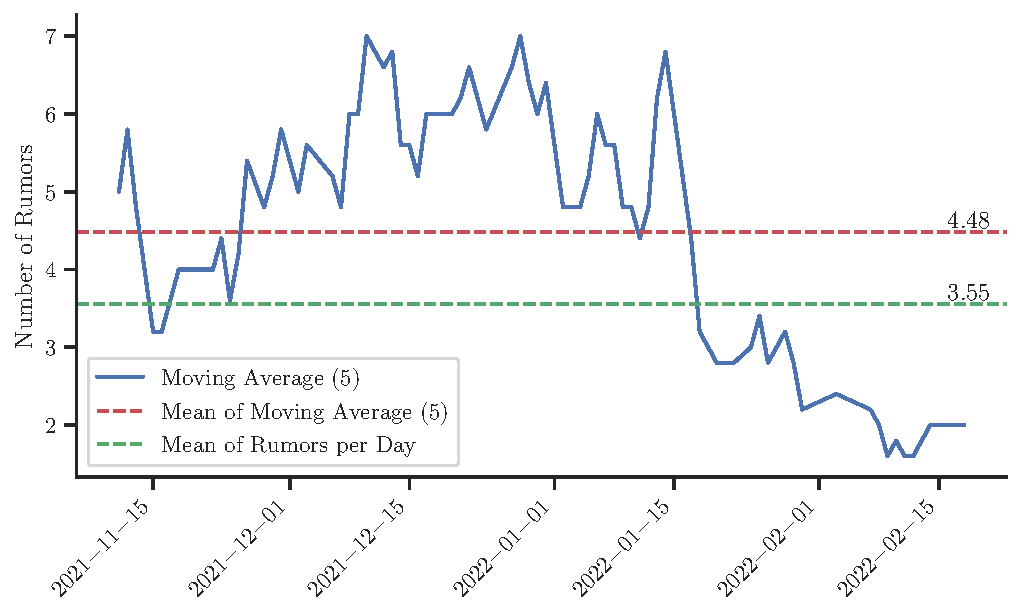
\includegraphics[width=0.6\linewidth]{../figures/rumor_num_ma5}
    \caption{不同日期的谣言数量(5日移动平均)}
    \label{fig:rumor_num_ma5}
\end{figure}

% 地理分布

图~\ref{fig:rumor_num_choropleth}~展示了各省市在数据集时间跨度内的谣言数量分布
%\footnote{Scale of rumor numbers为$\ln(\textrm{谣言数量} + 1)$,避免陕西和浙江过多的谣言数量影响视觉效果。图中各点大小没有做log处理。}
,从图中可以发现,谣言数量呈现三级分化:
西部地区谣言数量很少;华中谣言数量居中,但仍然较少;华北、华南地区谣言数量较多。

\begin{figure}[!ht]
    \centering
    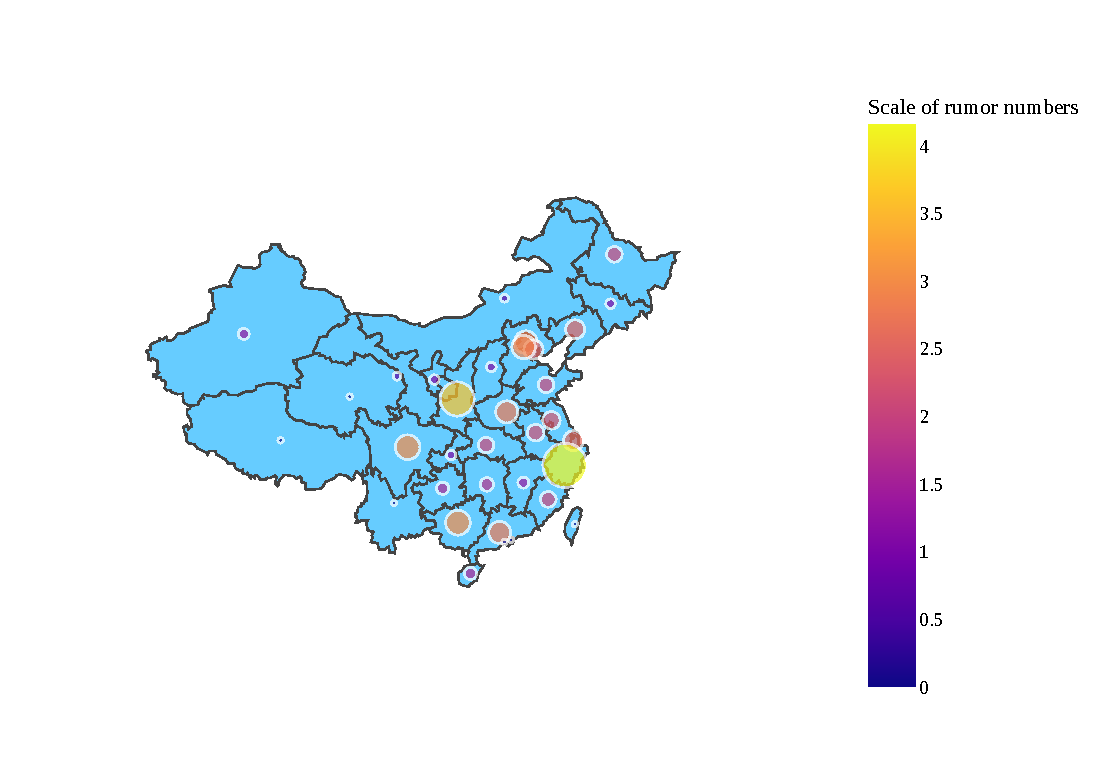
\includegraphics[width=0.6\linewidth]{../figures/rumor_num_choropleth}
    \caption{各省市谣言数量分布图}
    \label{fig:rumor_num_choropleth}
\end{figure}

%谣言数量的演化

图~\ref{fig:rumor_num_evolution}~展示了谣言数量的演化,从图中可以发现,谣言数量呈现如下趋势:
2021年11月四川的谣言最多,此外全国各地都有零星谣言,这可能和2021年11月13日起四川发生的疫情有关;
2021年12月浙江的谣言最多,此外,陕西也有较多的谣言,这可能和12月份浙江和陕西发生的疫情有关;
2022年1月起陕西、京津冀、浙江、广西等地的谣言均较多,这可能和2022年1月起这些地区发生的疫情有关。
可以发现,谣言数量的变化与疫情的演变有一定的关系,在之后的疫情相关分析中,我们也将更加详细地分析谣言数量与疫情的关系。

\begin{figure}[!ht]
    \begin{subfigure}[b]{0.3\textwidth}
         \centering
         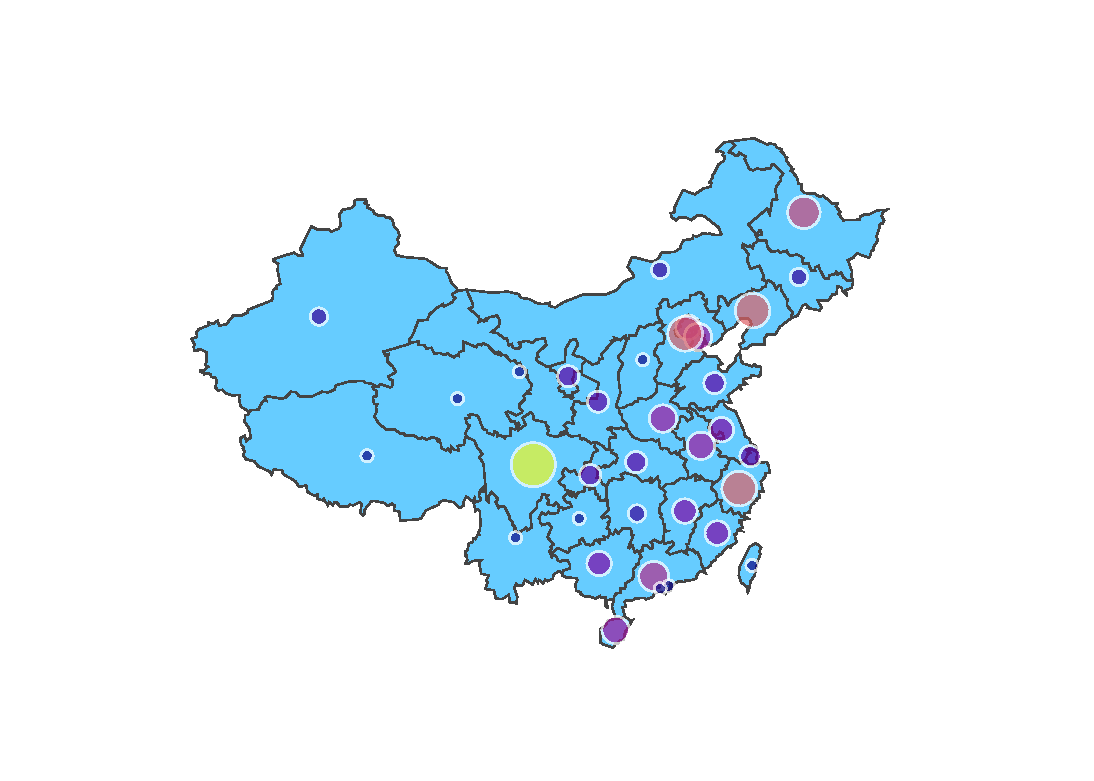
\includegraphics[width=\textwidth]{../figures/rumor_num_choropleth_0}
         \caption{2021-11-07至2021-12-07}
         \label{subfig:rumor_num_choropleth_0}
     \end{subfigure}
     \hfill
     \begin{subfigure}[b]{0.3\textwidth}
         \centering
         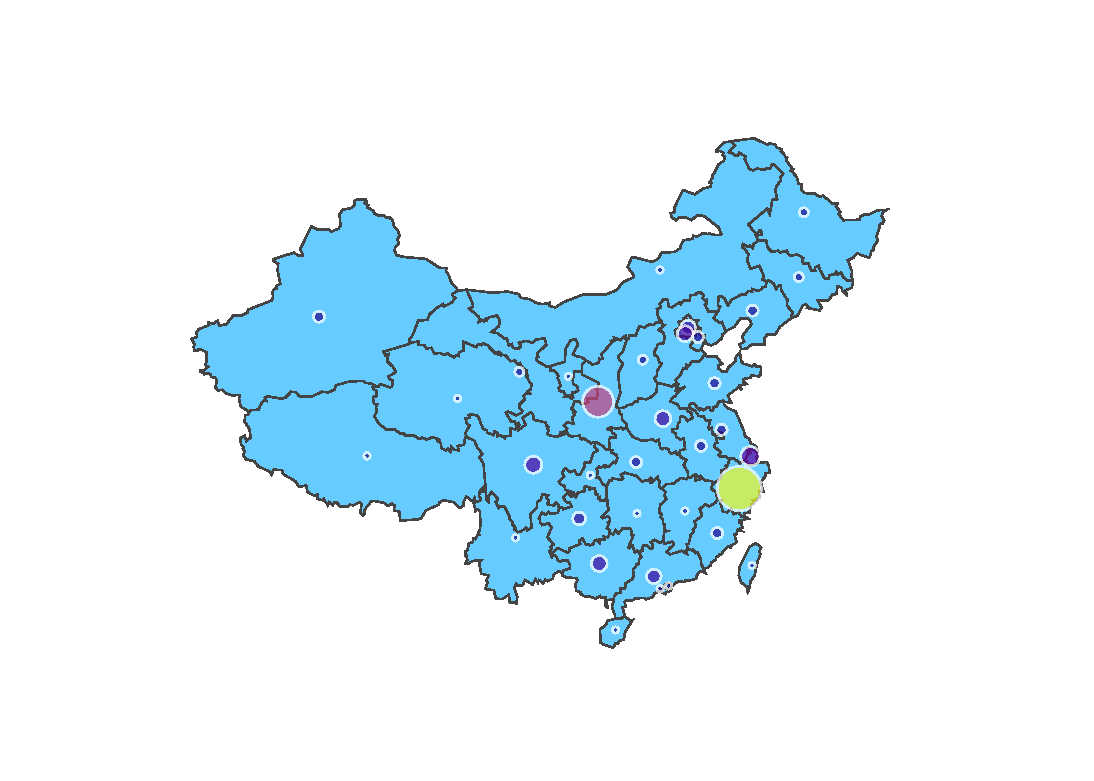
\includegraphics[width=\textwidth]{../figures/rumor_num_choropleth_1}
         \caption{2021-12-08至2022-01-07}
         \label{subfig:rumor_num_choropleth_1}
     \end{subfigure}
     \hfill
     \begin{subfigure}[b]{0.3\textwidth}
         \centering
         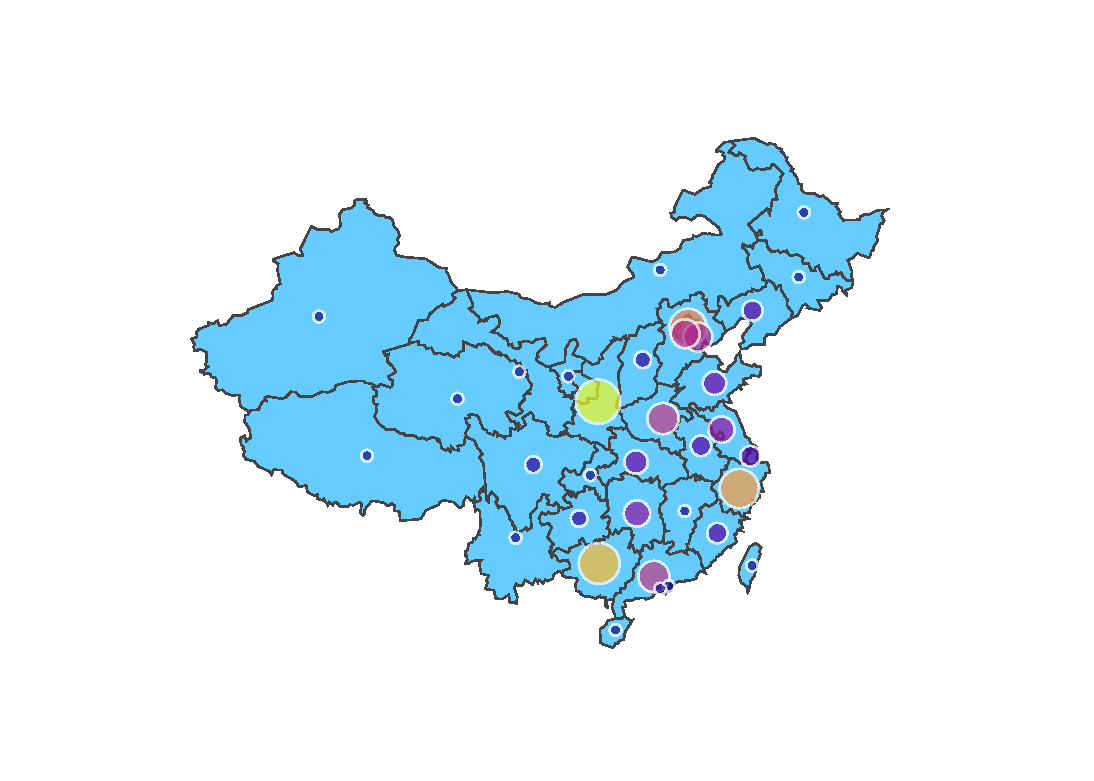
\includegraphics[width=\textwidth]{../figures/rumor_num_choropleth_2}
         \caption{2022-01-08至2022-02-18}
         \label{subfig:rumor_num_choropleth_2}
     \end{subfigure}
    \caption{谣言数量的演化}
    \label{fig:rumor_num_evolution}
\end{figure}

\subsection{文本分析}

利用\verb|jieba|库中\verb|jieba.analyse.extract_tags|方法,可以提取文本中的主题词。我们针对每条谣言内容提取3个主题词。
接下来,我们主要利用数据预处理时所得到的分词以及主题词进行分析。

首先,我们通过构建词云来展示分词以及主题词的构成,如图~\ref{fig:wordcloud}~所示。
由于数据库中谣言内容通常是辟谣时所呈现出的文字,所以无论是分词词云还是主题词词云,与辟谣相关的词语占据了很大的比重,
如“谣言”、“网传”、“造谣”、“核实”等;此外,和新冠疫情相关的词语也占据了很大的比重,
如“疫情”、“核酸”、“新冠”、“确诊”、“防控”等。
词云中所展示的词语大多为中性词,不能反映出谣言的特点,但是在谣言出现数量多的词可以反映出大部分谣言的主题,
可以分析出在谣言中哪些主题可能占比较高,疫情就是这些谣言中占比较高的主题之一。

\begin{figure}[!ht]
    \centering
    \begin{subfigure}[b]{0.45\textwidth}
        \centering
        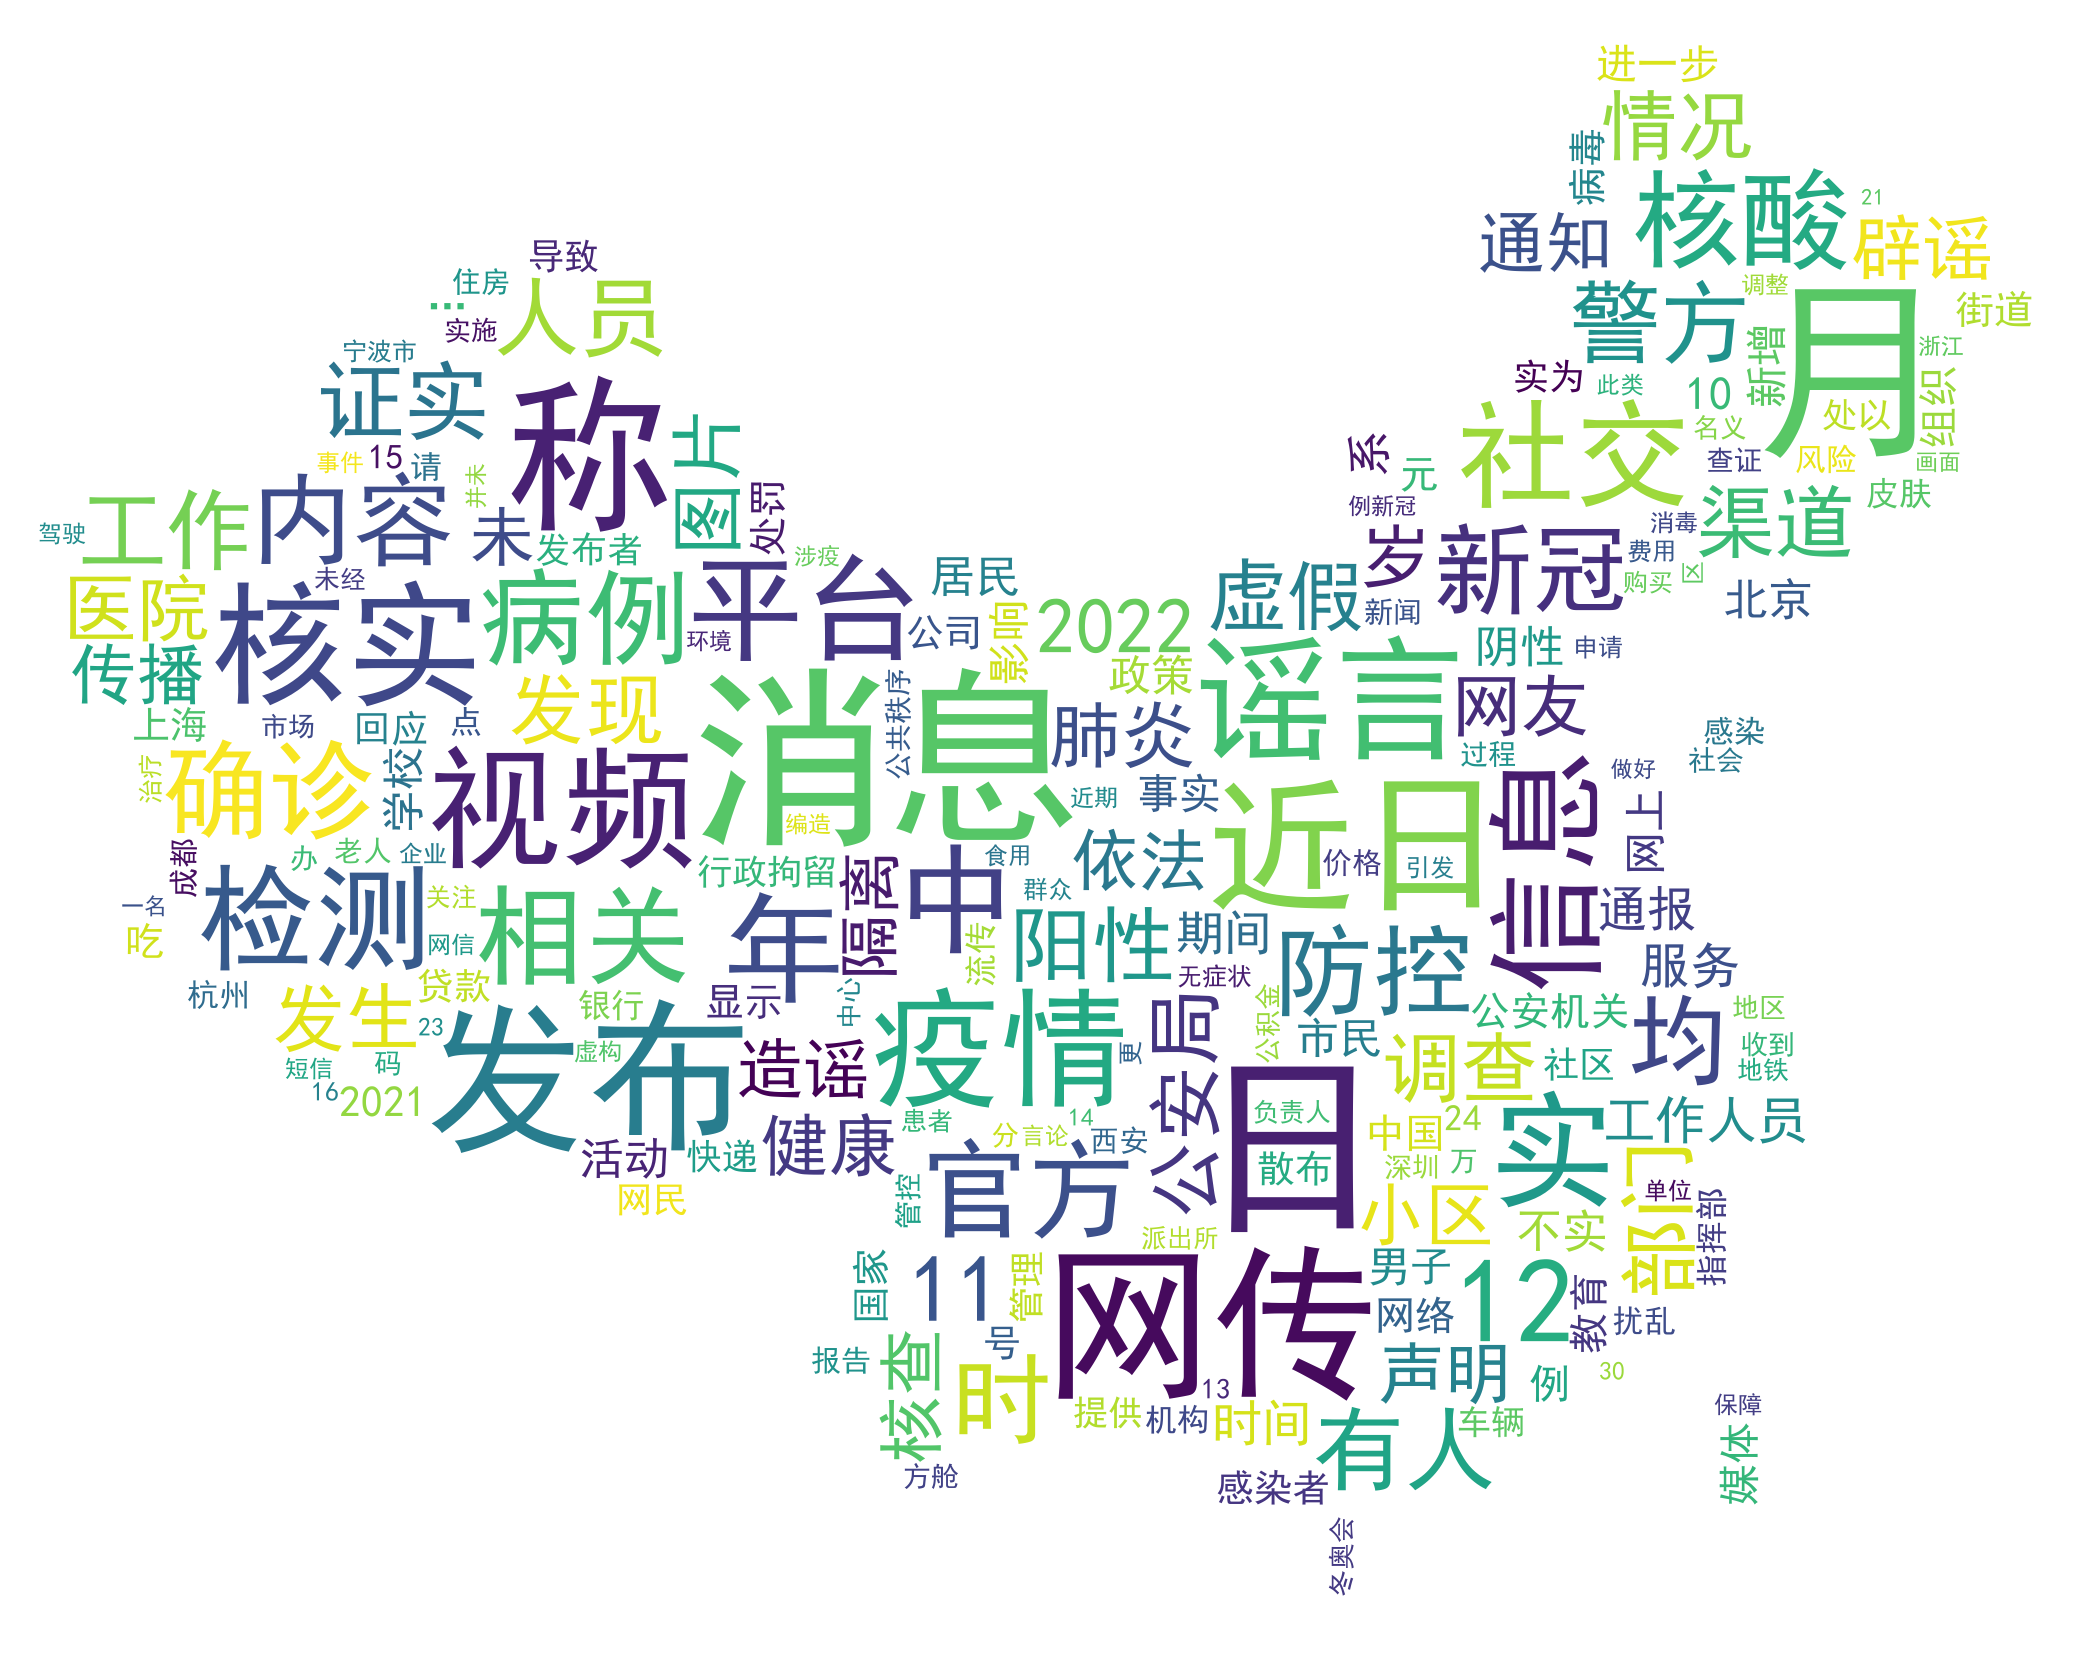
\includegraphics[width=\figwidth]{../figures/wordcloud_tokens}
        \caption{分词}
        \label{subfig:wordcloud_tokens}
    \end{subfigure}
    \hfill
    \begin{subfigure}[b]{0.45\textwidth}
        \centering
        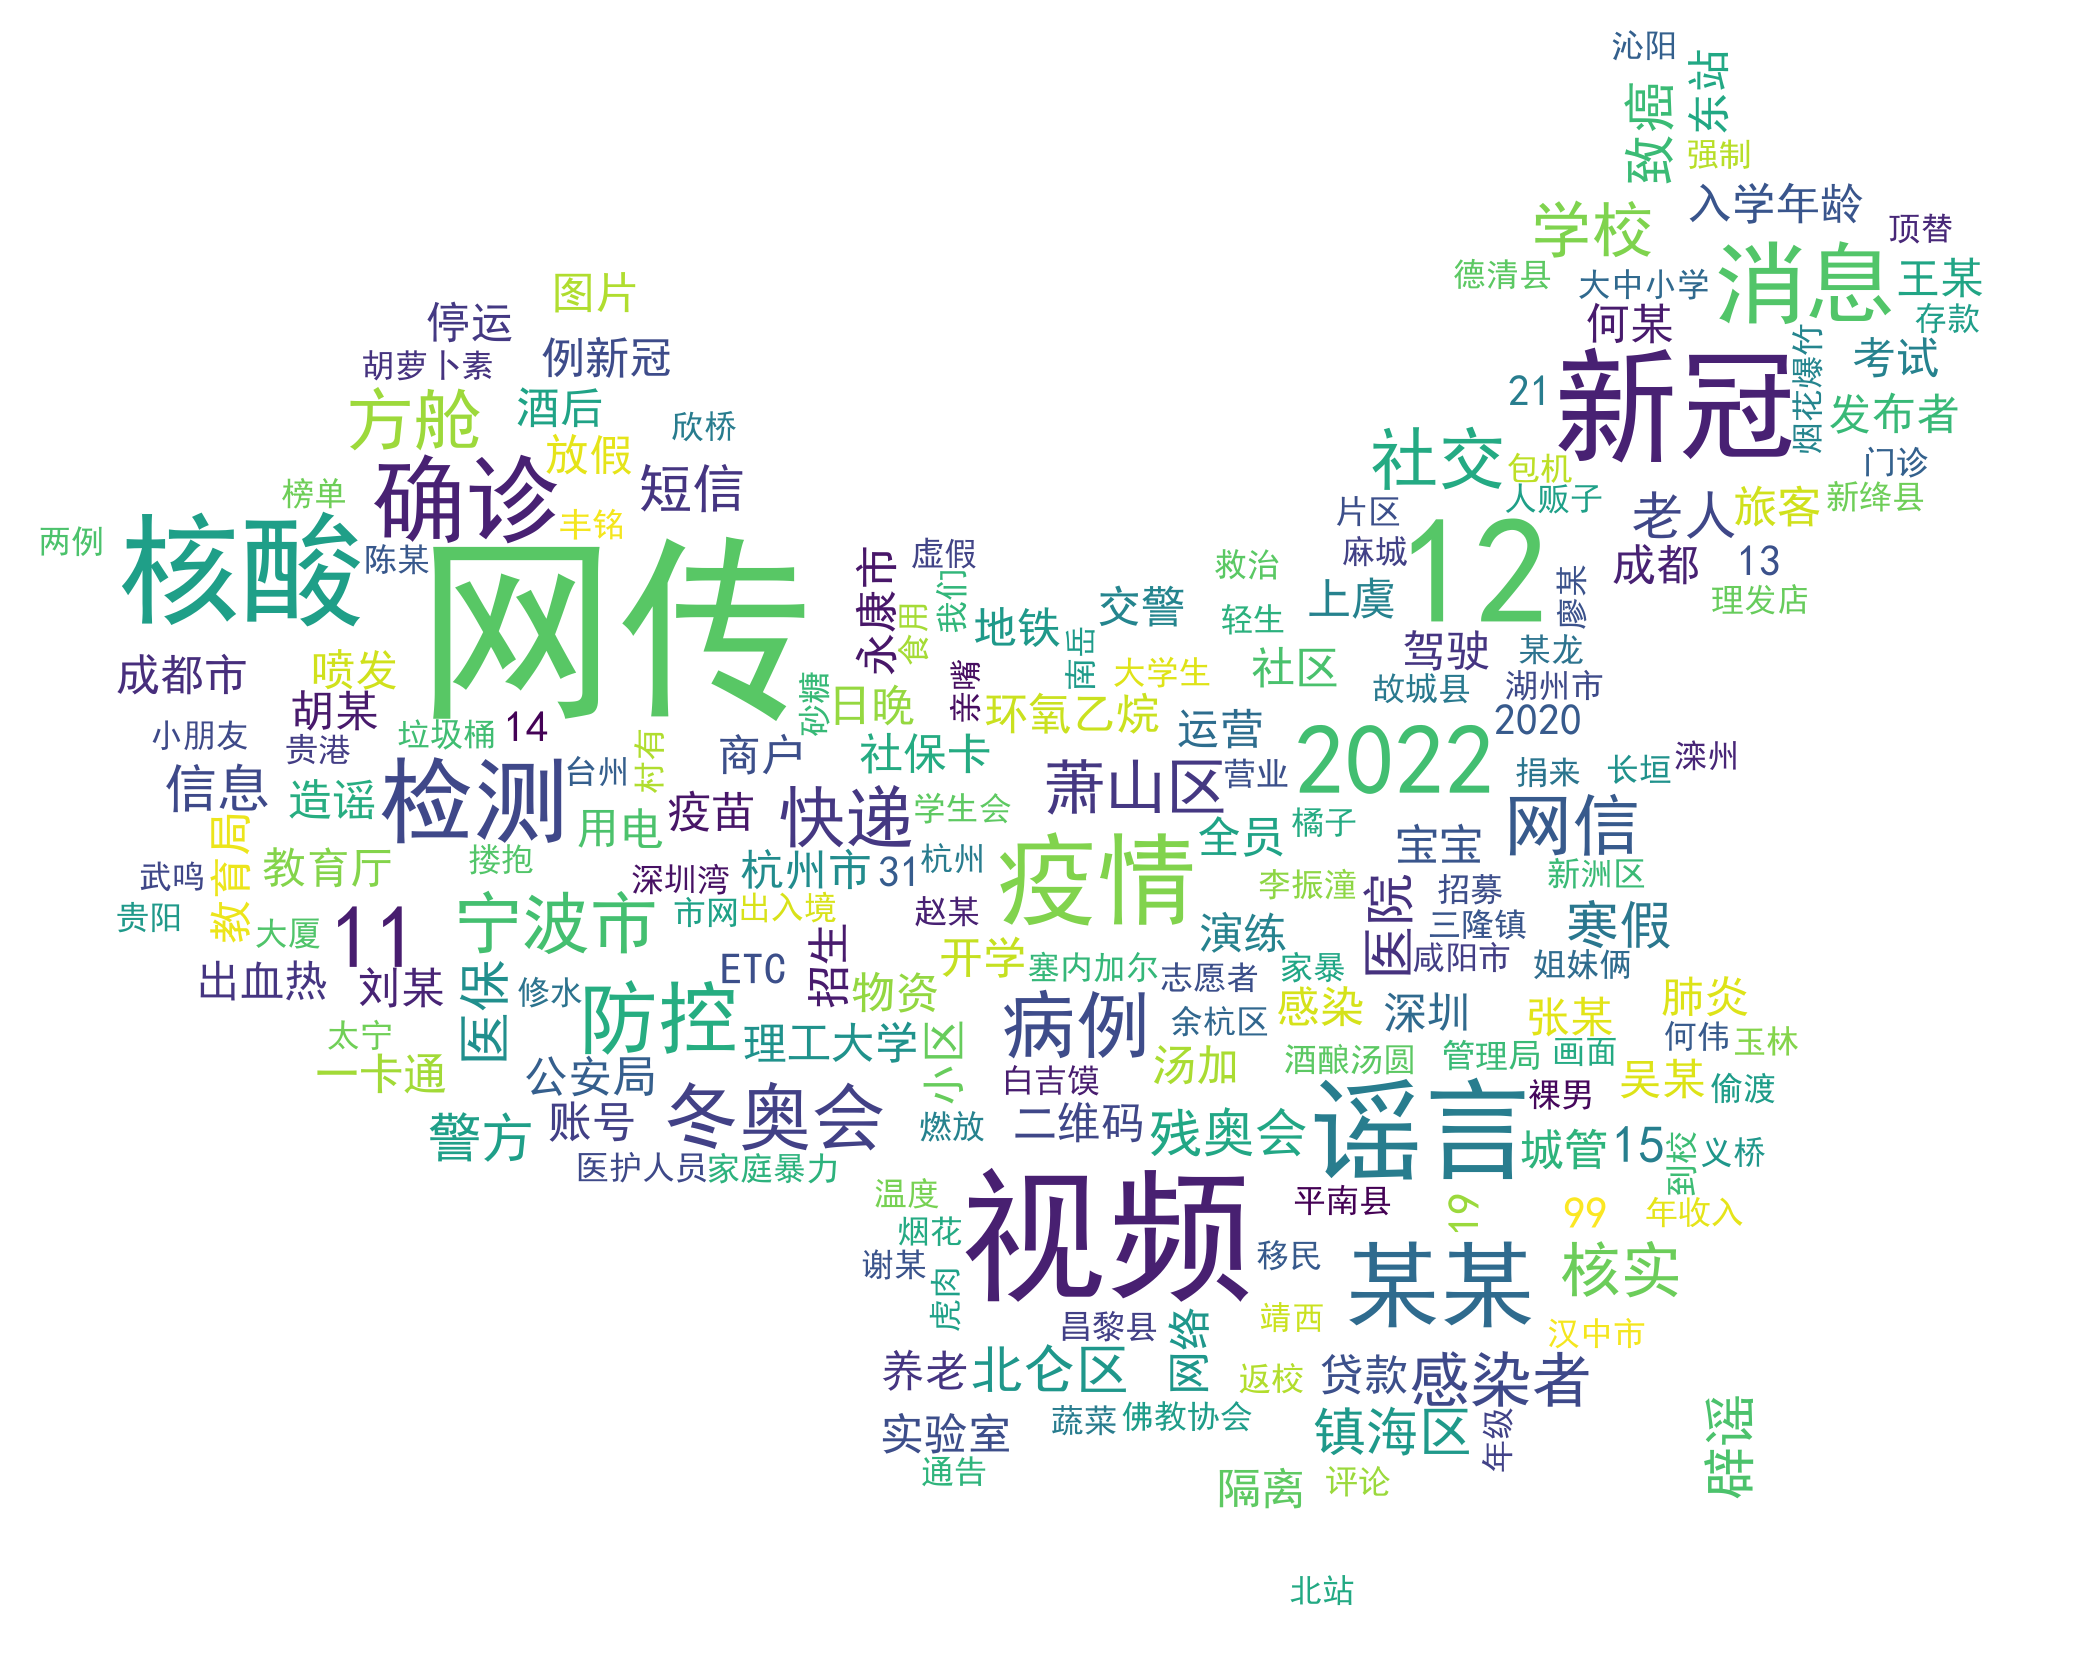
\includegraphics[width=\figwidth]{../figures/wordcloud_topics}
        \caption{主题词}
        \label{subfig:wordcloud_topics}
    \end{subfigure}
    \caption{词云}
    \label{fig:wordcloud}
\end{figure}

接下来,我们通过LDA方法进行主题挖掘,设定主题数为5并通过\verb|pyLDAvis|库进行可视化,结果如图~\ref{fig:LDAtopic}~和表~\ref{tab:LDAtopic}~所示。

\begin{figure}[!ht]
    \centering
    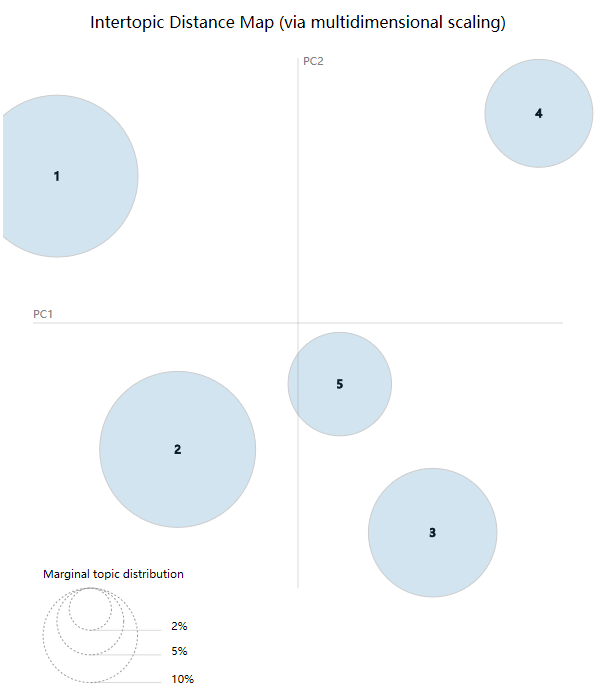
\includegraphics[width=0.45\linewidth]{../figures/LDAtopic}
    \caption{LDA方法得出的主题间距离}
    \label{fig:LDAtopic}
\end{figure}

\begin{table}[!ht]
    \centering
    \resizebox{1\columnwidth}{!}{
    \begin{tabular}{lr}
        \toprule
        \thead{\large{主题}} & \thead{\large{相关词语}} \\
        \midrule
        Default & \makecell{视频,平台,12,社交,月,日,近日,坚果,吃,公积金,小区,时,谣言,信息, \\ 皮肤,元,内容,陨石,食用,核实,甲醛,北京,群,图片,关节炎,检测,例,贷款,男子,警方} \\
        1 & \makecell{消息,月,网传,日,发布,称,近日,实,年,疫情,谣言,核实,视频,中,\\ 相关,12,官方,防控,确诊,信息,时,11,证实,内容,病例,核酸,检测,平台,均,2022} \\
        2 & \makecell{日,月,消息,发布,称,网传,近日,谣言,检测,信息,核实,疫情,社交,\\ 实,视频,平台,核酸,新冠,年,中,官方,均,病例,有人,相关,阳性,防控,医院,12,内容} \\
        3 & \makecell{月,消息,日,网传,称,12,核实,发布,谣言,检测,近日,确诊,病例,\\ 核酸,均,中,视频,疫情,实,社交,人员,小区,信息,相关,年,平台,新冠,11,时,官方} \\
        4 & \makecell{近日,消息,称,发布,日,社交,视频,月,平台,中,信息,网传,核实,\\ 谣言,内容,时,年,相关,官方,疫情,警方,12,检测,防控,男子,公安局,调查,实,渠道,活动} \\
        5 & \makecell{日,月,视频,称,消息,谣言,近日,发布,平台,核实,网传,信息,疫情,\\ 社交,内容,年,中,时,实,确诊,警方,有人,图片,相关,病例,12,元,官方,北京,发生} \\
        \bottomrule
    \end{tabular}
    }
    \caption{LDA方法得出的各主题前30个相关词语}
    \label{tab:LDAtopic}
\end{table}

%\noindent\begin{minipage}{\textwidth}
%    \begin{minipage}[b]{0.49\textwidth}
%        \centering
%        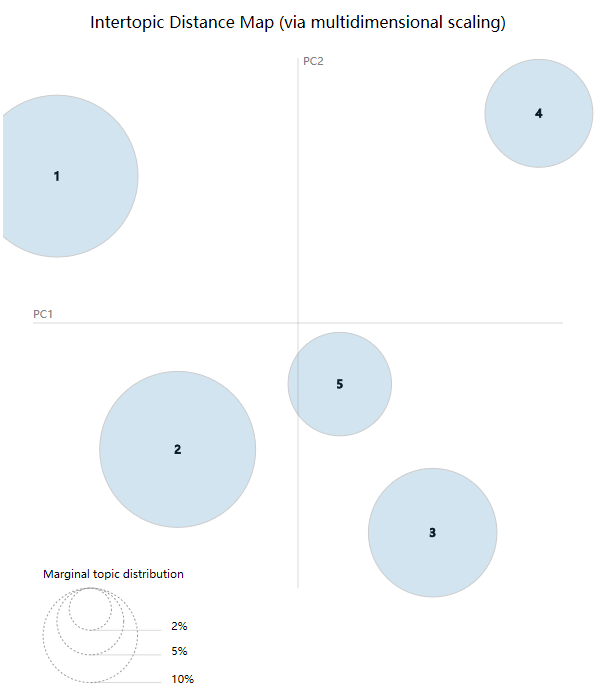
\includegraphics[width=0.85\linewidth]{../figures/LDAtopic}
%        \captionof{figure}{LDA方法得出的主题间距离}
%    \end{minipage}
%    \hfill
%    \begin{minipage}[b]{0.49\textwidth}
%    \centering
%        \begin{tabular}{lr}
%        \toprule
%        主题 & 相关词语 \\
%        \midrule
%        Default & \makecell{视频,平台,12,社交,月,日,近日,坚果,吃,公积金,小区,时,谣言,信息, \\ 皮肤,元,内容,陨石,食用,核实,甲醛,北京,群,图片,关节炎,检测,例,贷款,男子,警方} \\
%        1 & \makecell{消息,月,网传,日,发布,称,近日,实,年,疫情,谣言,核实,视频,中,\\ 相关,12,官方,防控,确诊,信息,时,11,证实,内容,病例,核酸,检测,平台,均,2022} \\
%        2 & \makecell{日,月,消息,发布,称,网传,近日,谣言,检测,信息,核实,疫情,社交,\\ 实,视频,平台,核酸,新冠,年,中,官方,均,病例,有人,相关,阳性,防控,医院,12,内容} \\
%        3 & \makecell{月,消息,日,网传,称,12,核实,发布,谣言,检测,近日,确诊,病例,\\ 核酸,均,中,视频,疫情,实,社交,人员,小区,信息,相关,年,平台,新冠,11,时,官方} \\
%        4 & \makecell{近日,消息,称,发布,日,社交,视频,月,平台,中,信息,网传,核实,\\ 谣言,内容,时,年,相关,官方,疫情,警方,12,检测,防控,男子,公安局,调查,实,渠道,活动} \\
%        5 & \makecell{日,月,视频,称,消息,谣言,近日,发布,平台,核实,网传,信息,疫情,\\ 社交,内容,年,中,时,实,确诊,警方,有人,图片,相关,病例,12,元,官方,北京,发生} \\
%        \bottomrule
%        \end{tabular}
%    \captionof{table}{LDA方法得出的各主题前30个相关词语}
%    \end{minipage}
%\end{minipage}

从图~\ref{fig:LDAtopic}~中可以看出,各主题之间都有一定的距离,说明各主题之间是有区分度的;
然而,从表~\ref{tab:LDAtopic}~中可以看出,主题1至5中,大部分词语都是相同的,如“月”、“日”、“谣言”等词,
而有区分度的词也不明显,如主题1中的、“防控”、“核酸”等词,主题2中的“阳性”、“医院”等词,都和疫情相关;
真正有区分度的词语(即不是含义不大、疫情相关的词)有
主题4中的“男子”、“公安局”、“警方”、“活动”等词,主题5中的“北京”、“警方”等词。

\subsection{用户分析}

在数据集中,有18位用户针对每条谣言是否浏览的记录,我们将对这18位用户进行分析。

首先,我们通过网络图展示18位用户之间的关系。每位用户为一个节点,如果两个用户浏览了相同的谣言,则这两个用户之间有一条边,
然后通过Louvain方法将用户分为不同的社区,最后将社区内的用户用不同的颜色标记。
结果如图~\ref{fig:user_network}~所示。可以发现,用户之间的关系可以被分为3个社区,社区1由用户0,2,6,7,8,11,12组成;
社区2由用户1,4,5,10,16组成;社区3由用户3,9,13,14,15,17组成。

\begin{figure}[!ht]
    \centering
    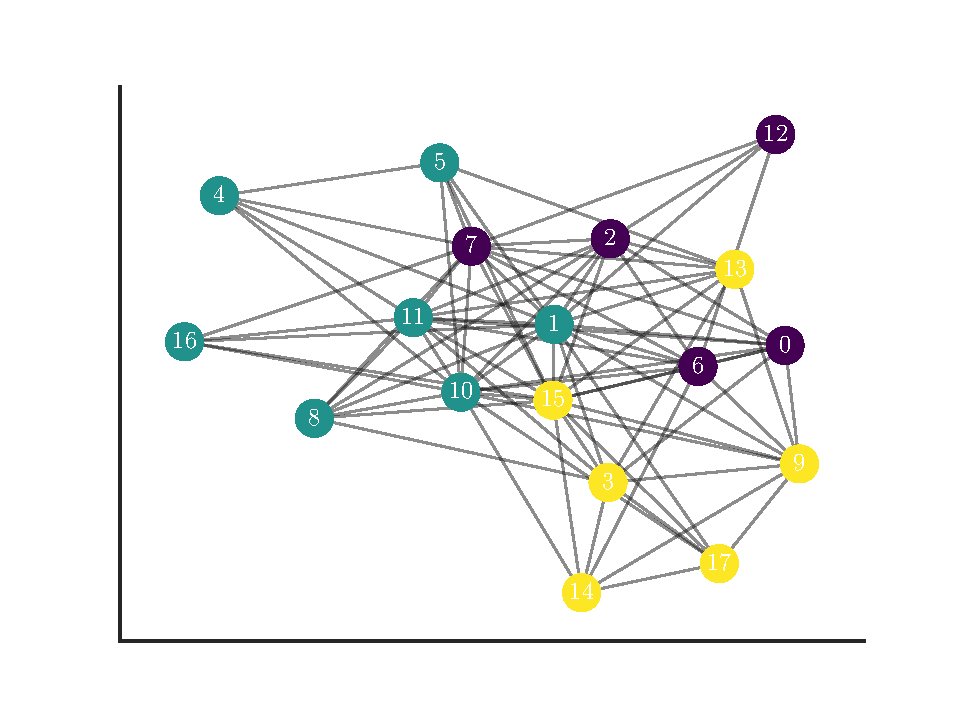
\includegraphics[width=0.6\linewidth]{../figures/user_network}
    \caption{用户网络图}
    \label{fig:user_network}
\end{figure}

我们假设单一社区内用户的浏览行为相似,通过将社区内用户浏览过的所有谣言合并在一起分析,我们可以尝试分析用户的浏览行为。
图~\ref{fig:wordcloud_user}~展示了不同社区内用户浏览谣言的主题词词云。
从图中可以看出,社区1和社区2中的用户主要浏览的谣言都和疫情有关,如“疫情”、“核酸”等词语在浏览谣言中的比重都很大;
而社区3中的用户主要浏览的谣言和疫情关系不是很大,虽然也有“疫情”、“医院”等词语,但比重不大,
而像“家庭暴力”、“酒后”、“考试”这类和生活相关的词语有一定的比重。在社区1和社区2中,和疫情相关的词语也有一定的区分度,
社区1中用户注重“确诊”、“病例”等和疫情发展有关的词语,而社区2中用户注重“核酸”、“检测”等和疫情防控有关的词语。

\begin{figure}[!ht]
    \begin{subfigure}[b]{0.3\textwidth}
         \centering
         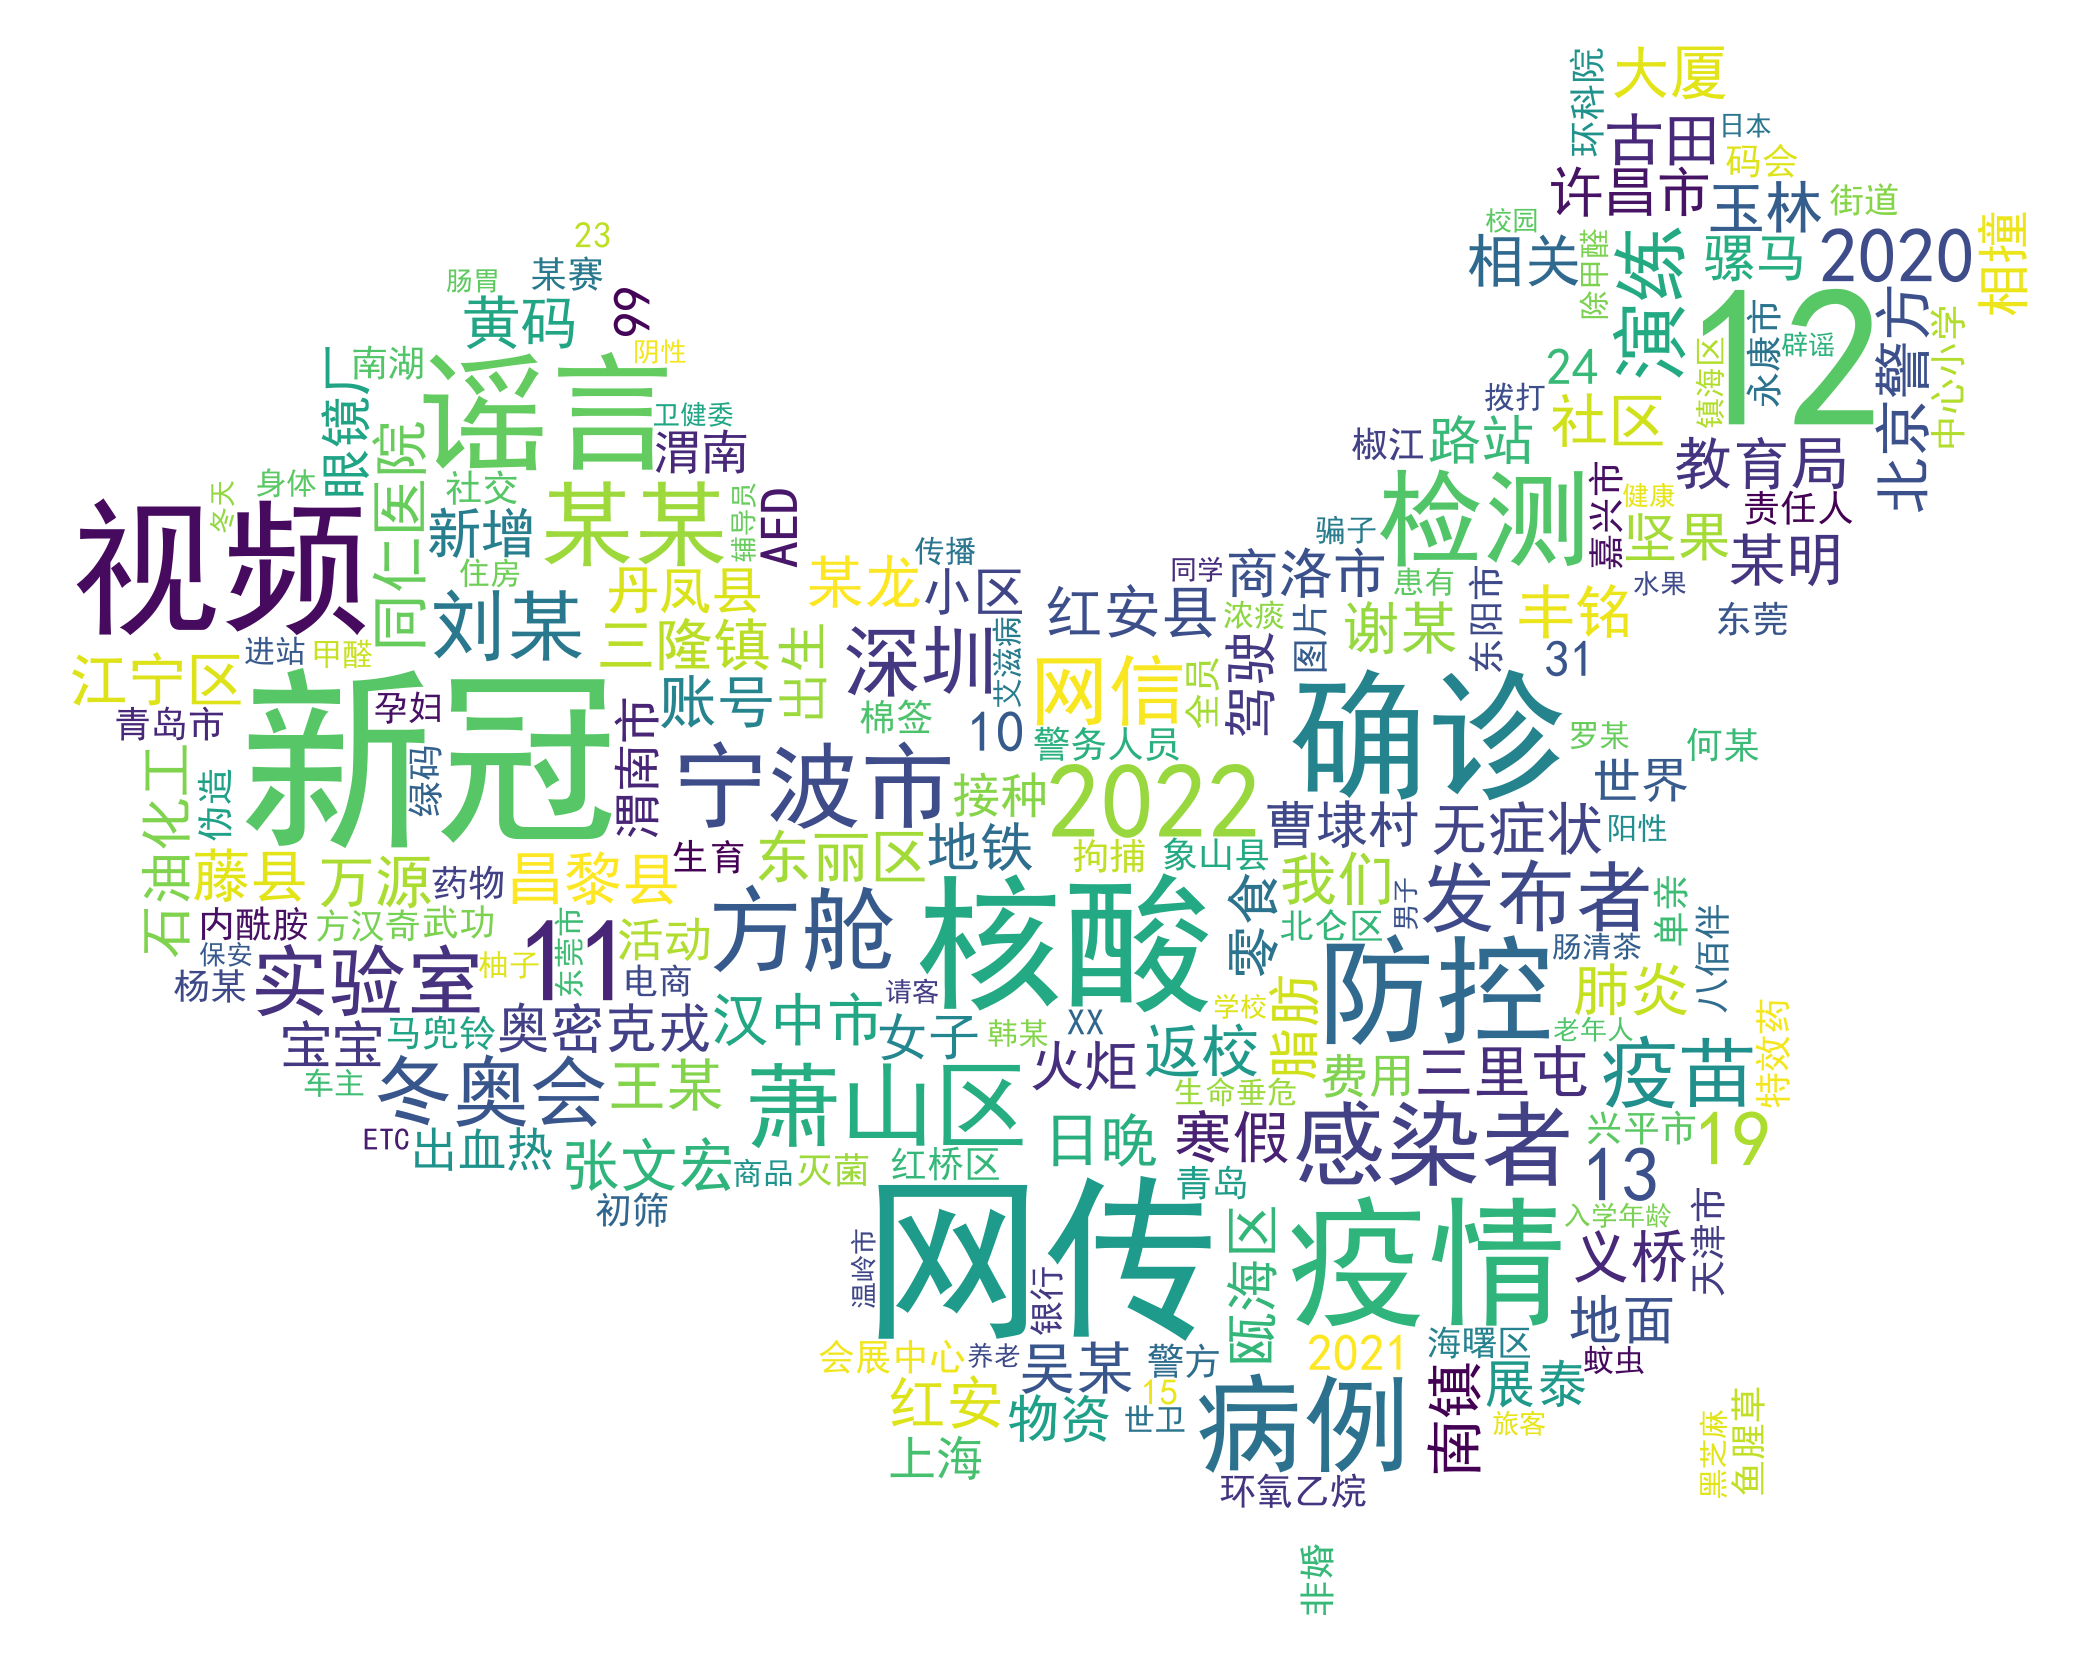
\includegraphics[width=\textwidth]{../figures/wordcloud_user_1}
         \caption{社区1用户}
         \label{subfig:wordcloud_user_1}
     \end{subfigure}
     \hfill
     \begin{subfigure}[b]{0.3\textwidth}
         \centering
         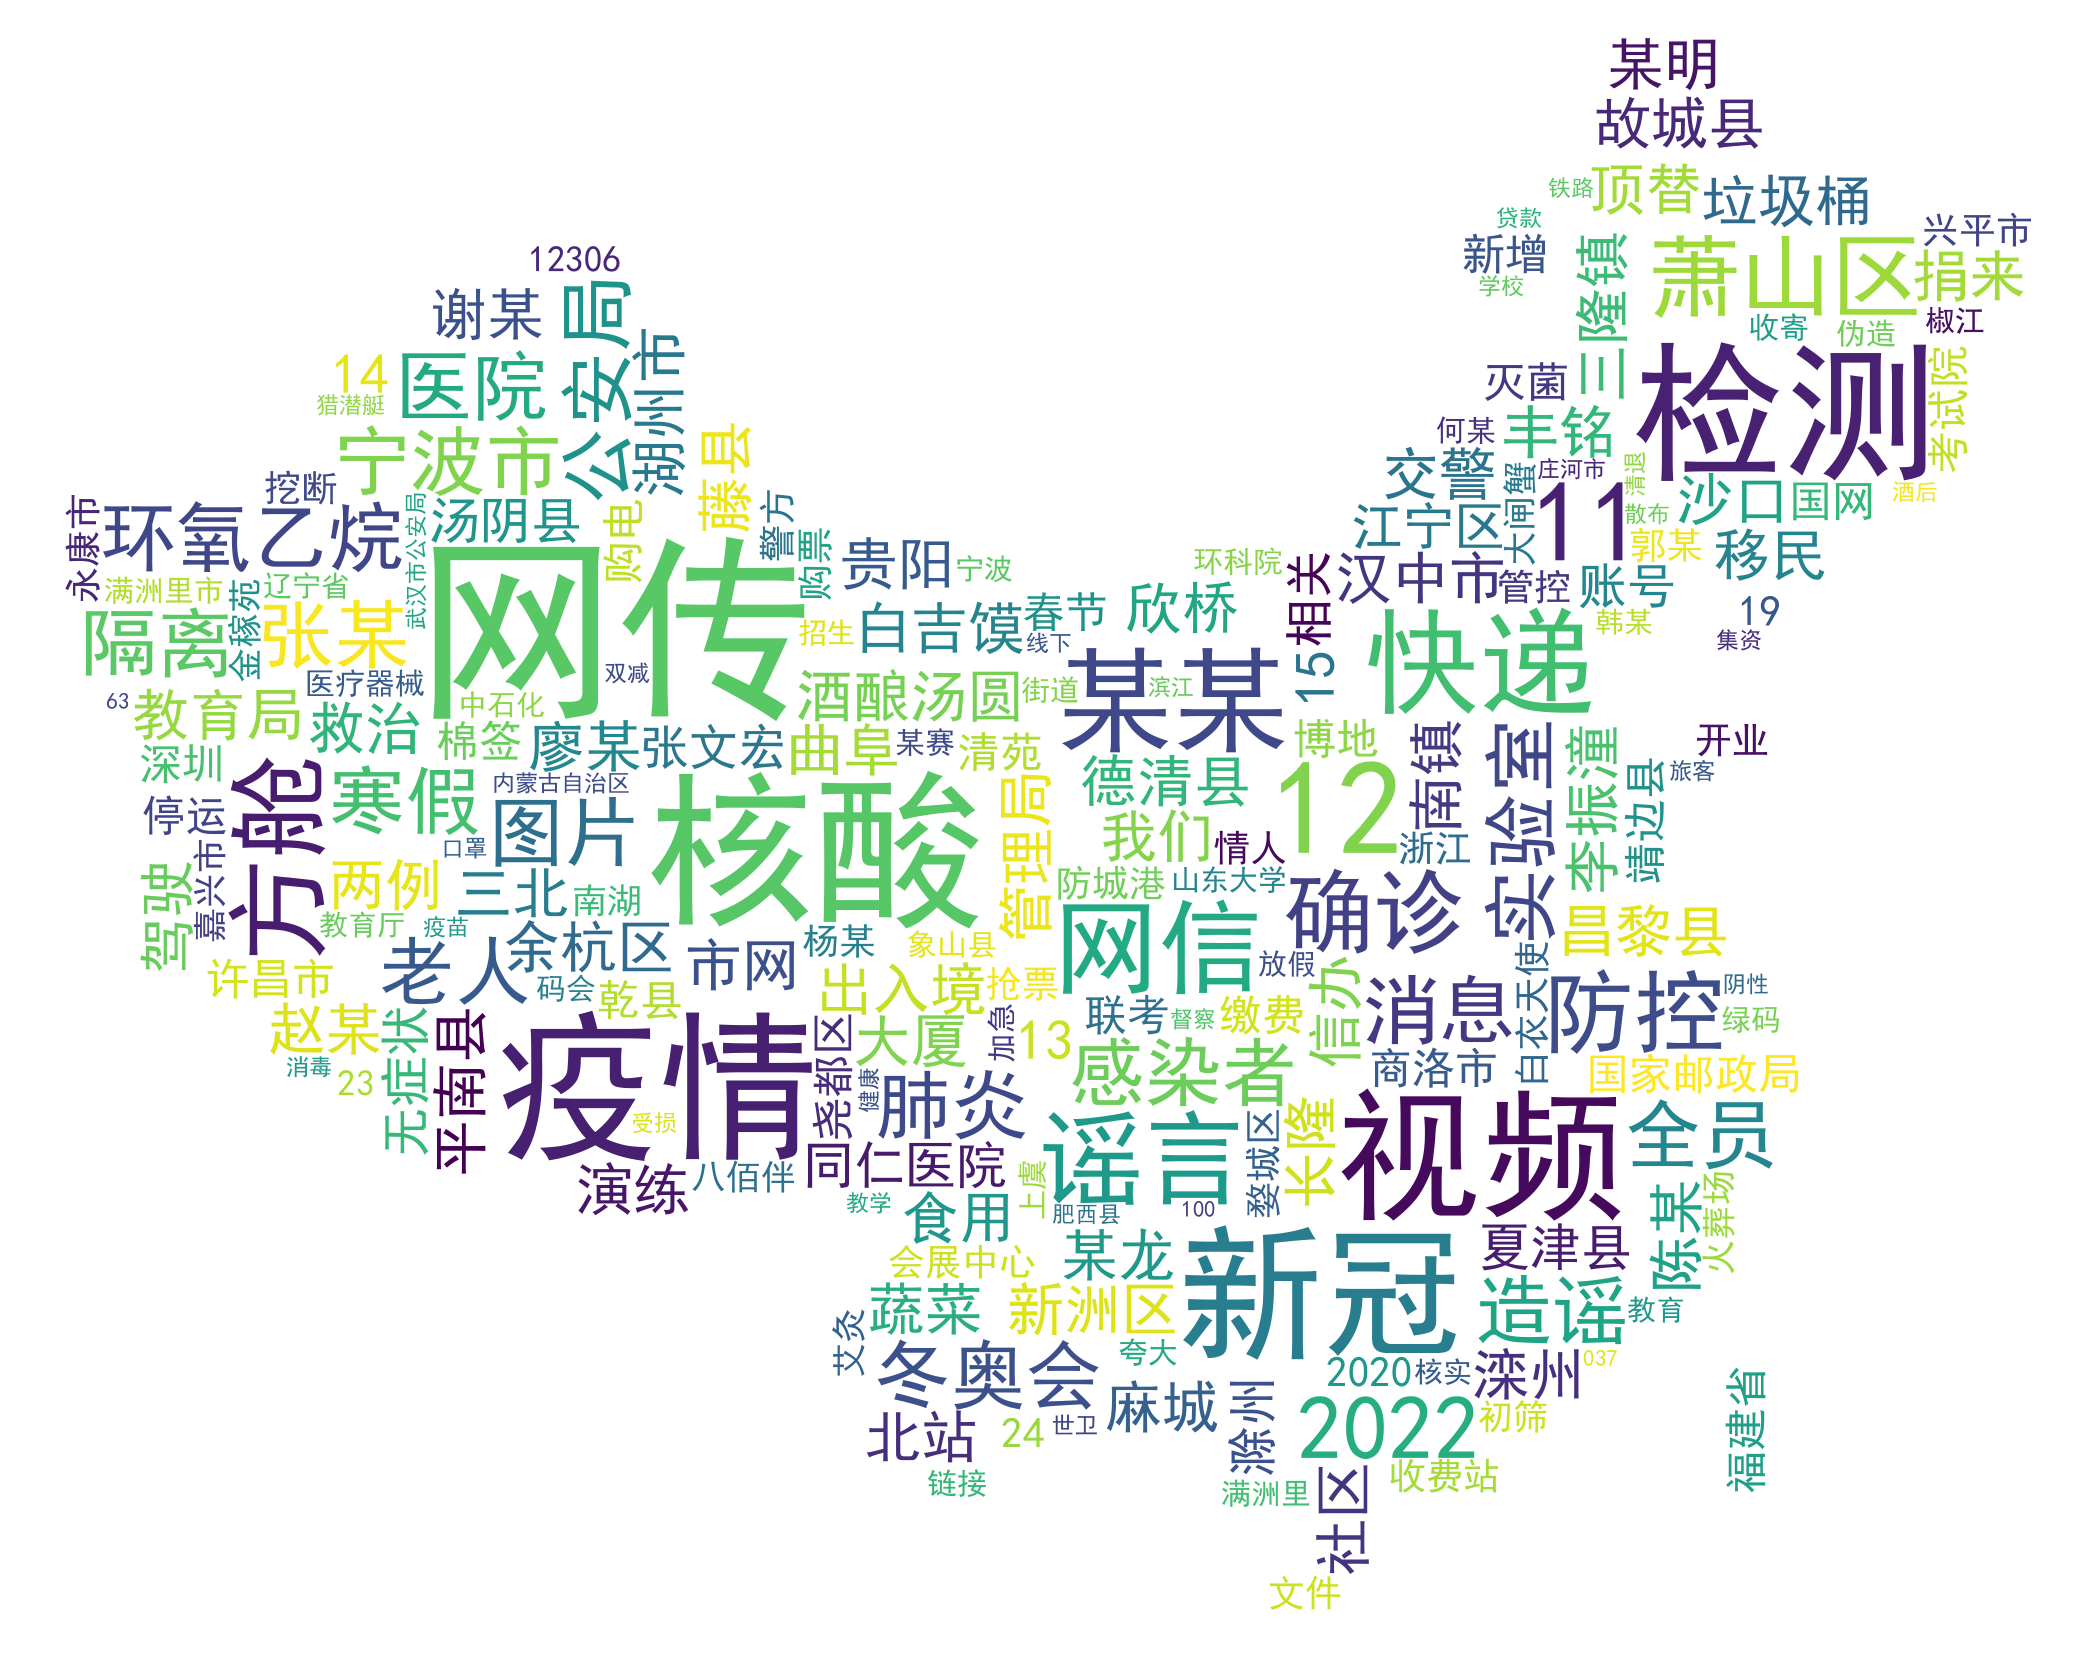
\includegraphics[width=\textwidth]{../figures/wordcloud_user_2}
         \caption{社区2用户}
         \label{subfig:wordcloud_user_2}
     \end{subfigure}
     \hfill
     \begin{subfigure}[b]{0.3\textwidth}
         \centering
         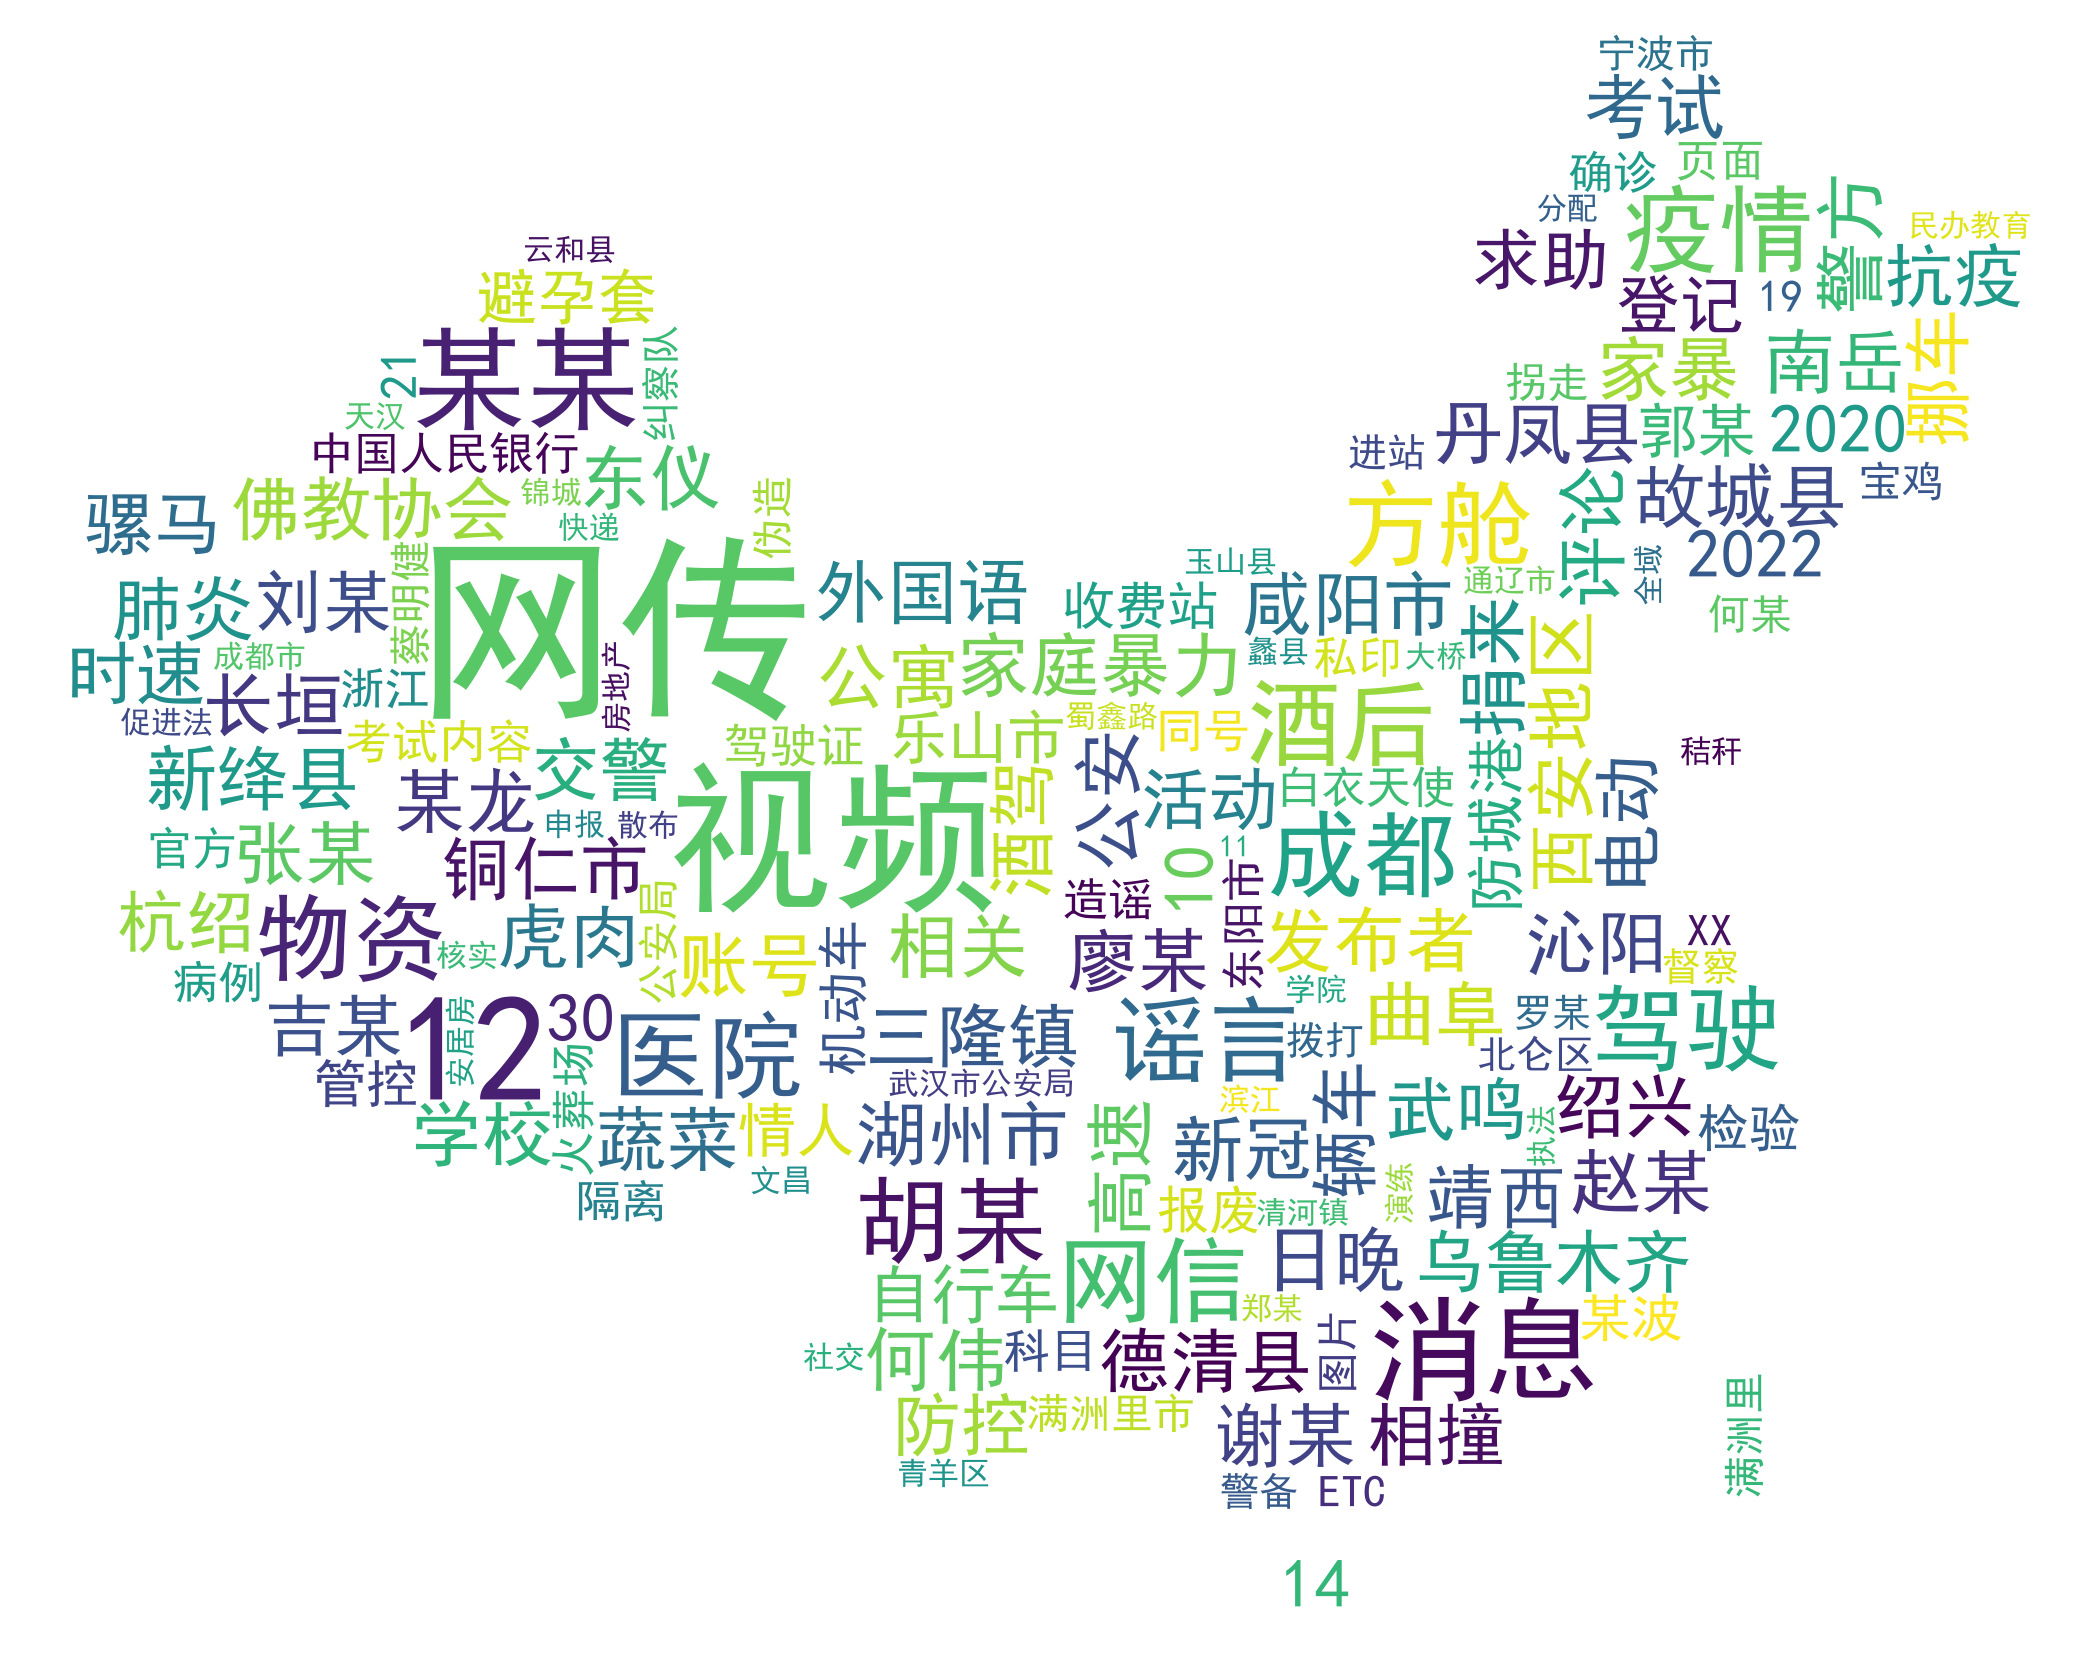
\includegraphics[width=\textwidth]{../figures/wordcloud_user_3}
         \caption{社区3用户}
         \label{subfig:wordcloud_user_3}
     \end{subfigure}
    \caption{各社区用户浏览谣言的主题词词云}
    \label{fig:wordcloud_user}
\end{figure}

\subsection{疫情相关分析}

这一部分我们将分析谣言与疫情的关系。首先我们需要把与疫情相关的谣言筛选出来。通过文本分析中的词云和LDA方法,
提取与疫情谣言相关的主题词\footnote{词语为: \textit{新冠, 疫情, 病毒, 疫苗, 病例, 确诊, 核酸, 防控},这里提取疫情谣言的方法可能会造成一定的误差。},
进而获得了与疫情相关的谣言166条,占总谣言数的45\%。

图~\ref{fig:covid_ma5}~展示了疫情谣言和非疫情谣言在不同日期的数量。
可以发现,疫情谣言呈现明显的高峰和低谷,而非疫情谣言的数量则大致呈现平稳下降趋势。
在11月底时,疫情谣言落入低谷,而非疫情谣言数量达到了最高峰,这可能是因为当时全国疫情得到控制,人们开始关注疫情以外的事情;
从12月开始到2022年1月中旬,疫情谣言除了在元旦期间有所回落,其余时间都维持高位,这是因为12月开始疫情开始在全国多地出现反弹,到1月中旬后,疫情才逐渐得到控制;
非疫情谣言则在12月中旬后迎来一波上升的小高峰,到1月中旬后开始下降,这可能是因为临近新年、寒假,生活上的谣言有所增加。

\begin{figure}[!ht]
    \centering
    \begin{subfigure}[b]{0.45\textwidth}
        \centering
        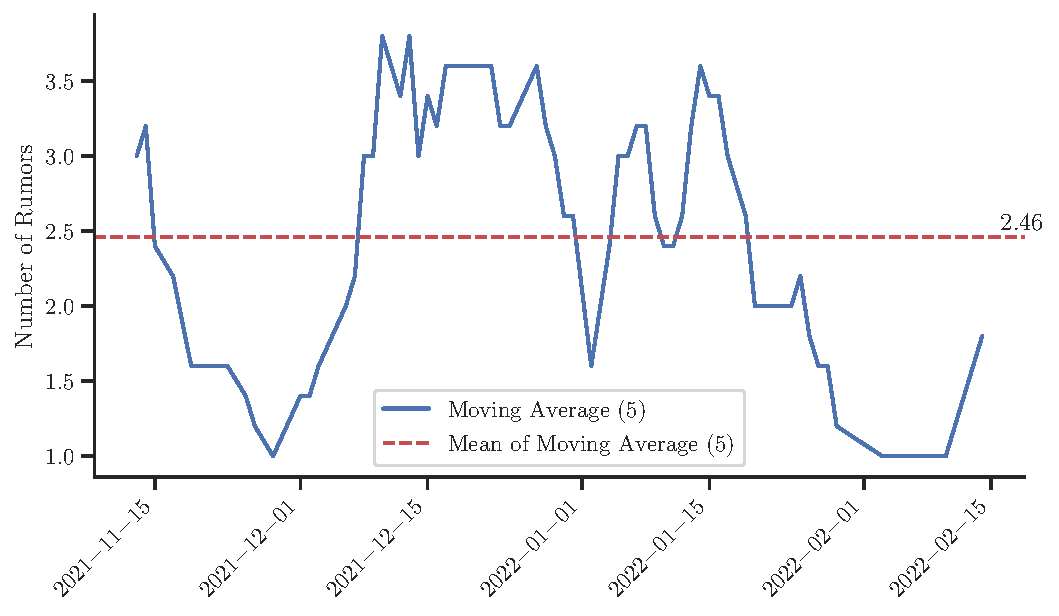
\includegraphics[width=\figwidth]{../figures/covid_rumor_num_ma5}
        \caption{疫情}
        \label{subfig:covid_ma5}
    \end{subfigure}
    \hfill
    \begin{subfigure}[b]{0.45\textwidth}
        \centering
        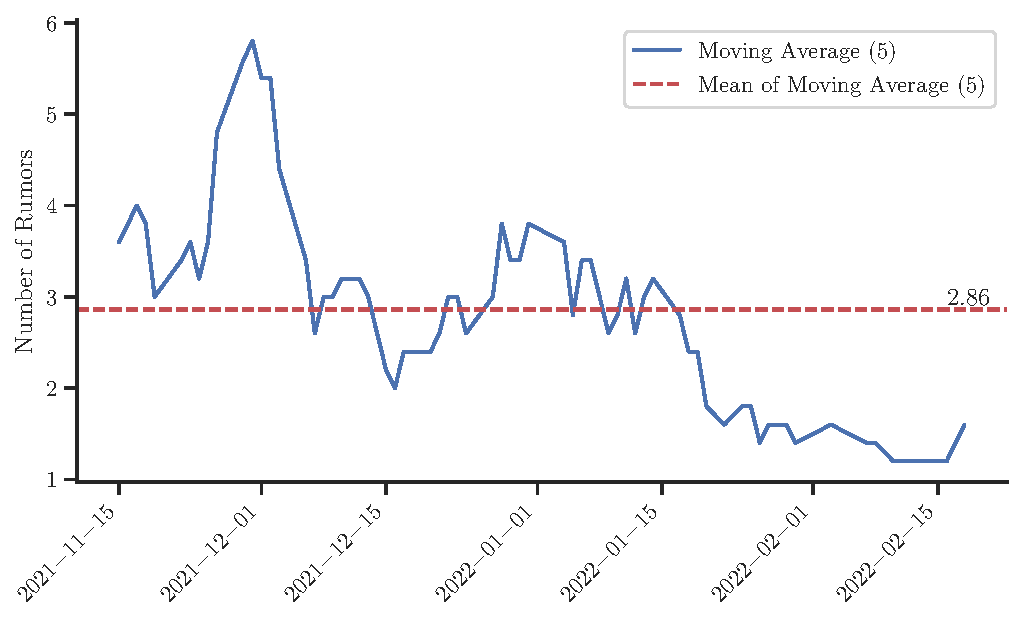
\includegraphics[width=\figwidth]{../figures/covid_no_rumor_num_ma5}
        \caption{非疫情}
        \label{subfig:no_covid_ma5}
    \end{subfigure}
    \caption{不同日期的谣言数量(5日移动平均)}
    \label{fig:covid_ma5}
\end{figure}

图~\ref{fig:covid_rumor_num}~展示了疫情谣言和非疫情谣言在数据集所有时间内的数量分布。
从图中可以看出,疫情谣言主要集中在浙江、陕西、四川、广西,这些地方也是有疫情发生的地方;
而非疫情谣言除了西部地区几乎没有谣言,在其余地区分布比较均匀。
注意,虽然从图上好像看似疫情谣言和非疫情谣言数量在浙江是一样多的,
但是浙江的疫情谣言数量有48,非疫情谣言数量只有17,相差很大,
这是由于表示谣言数量的点的最大大小和最强颜色跟随数量最大值走的。

\begin{figure}[!ht]
    \centering
    \begin{subfigure}[b]{0.45\textwidth}
        \centering
        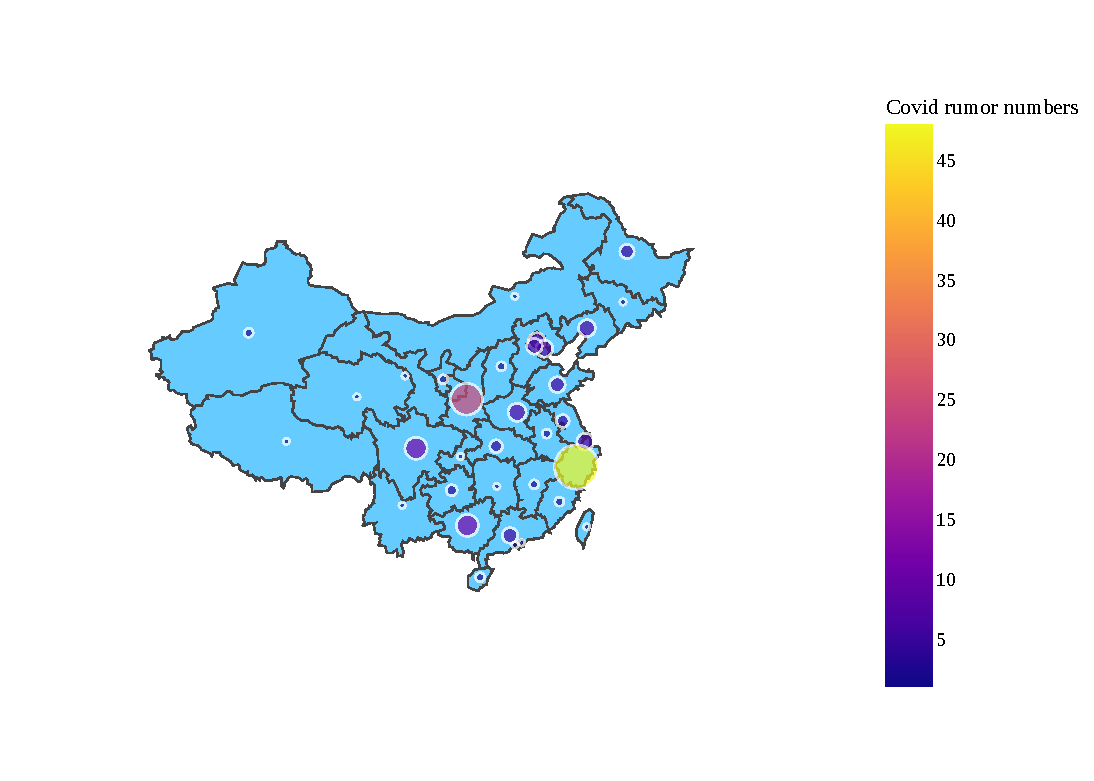
\includegraphics[width=\figwidth]{../figures/covid_rumor_num_choropleth}
        \caption{疫情}
        \label{subfig:covid_rumor_num}
    \end{subfigure}
    \hfill
    \begin{subfigure}[b]{0.45\textwidth}
        \centering
        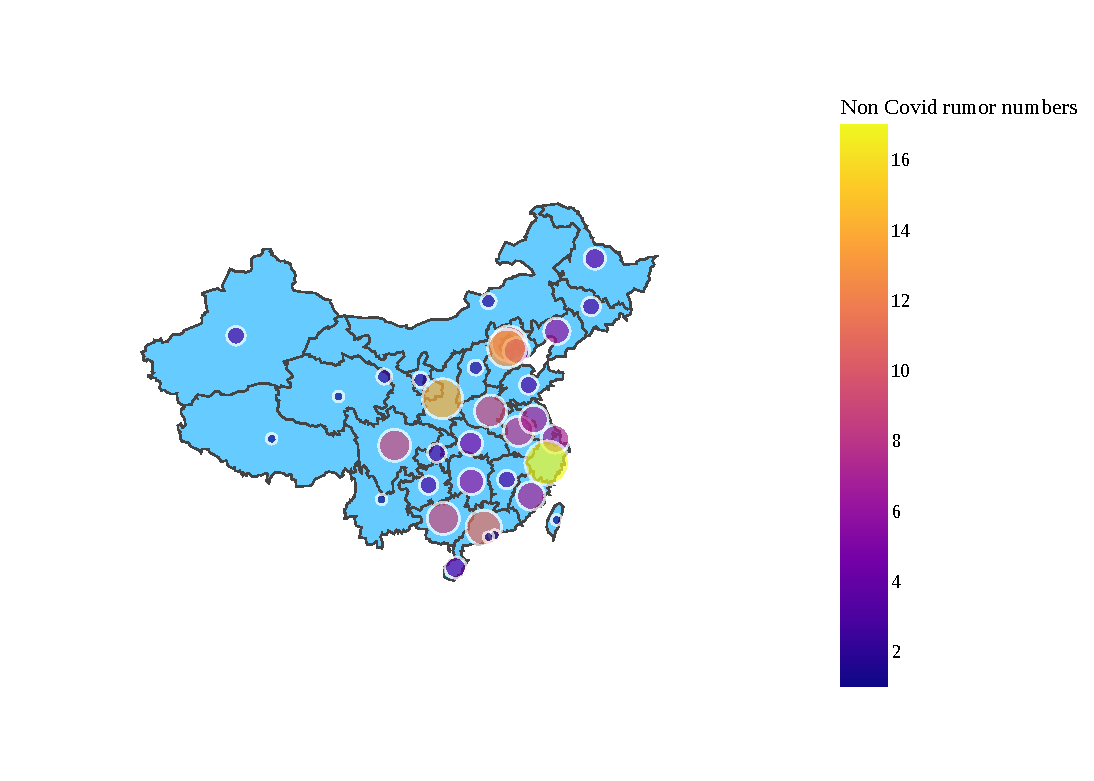
\includegraphics[width=\figwidth]{../figures/covid_no_rumor_num_choropleth}
        \caption{非疫情}
        \label{subfig:no_covid_rumor_num}
    \end{subfigure}
    \caption{各省市谣言数量分布}
    \label{fig:covid_rumor_num}
\end{figure}

图~\ref{fig:covid_rumor_num_evolution}~展示了疫情谣言在不同时间段的数量分布。
这里和一开始谣言数量分析时图~\ref{fig:rumor_num_evolution}~很相似,也就是说,疫情是主导谣言地域分布的主要因素。

\begin{figure}[!ht]
    \begin{subfigure}[b]{0.3\textwidth}
         \centering
         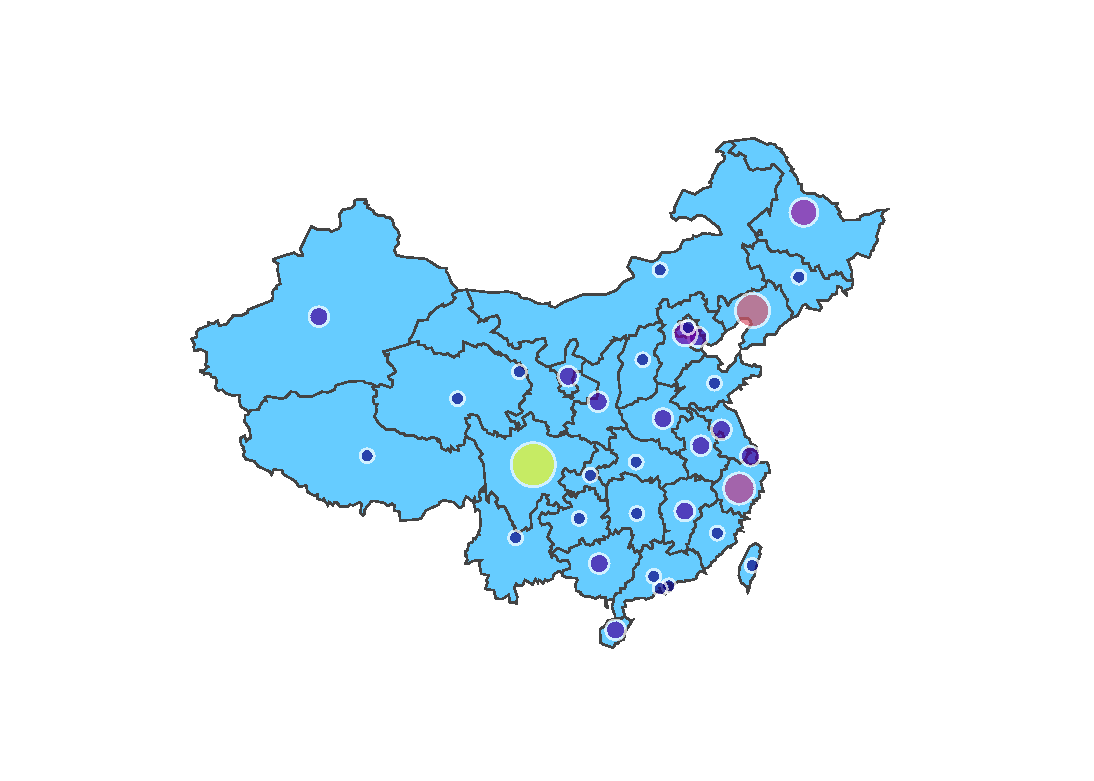
\includegraphics[width=\textwidth]{../figures/covid_rumor_num_choropleth_0}
         \caption{2021-11-07至2021-12-07}
         \label{subfig:covid_rumor_num_choropleth_0}
     \end{subfigure}
     \hfill
     \begin{subfigure}[b]{0.3\textwidth}
         \centering
         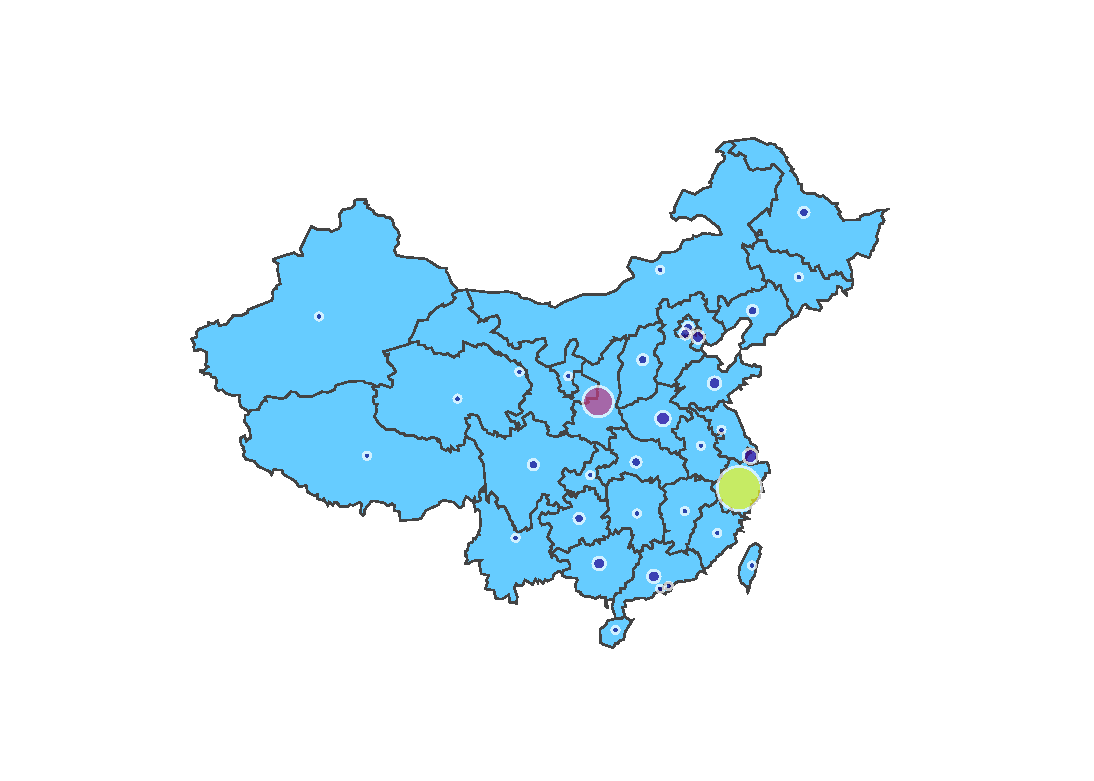
\includegraphics[width=\textwidth]{../figures/covid_rumor_num_choropleth_1}
         \caption{2021-12-08至2022-01-07}
         \label{subfig:covid_rumor_num_choropleth_1}
     \end{subfigure}
     \hfill
     \begin{subfigure}[b]{0.3\textwidth}
         \centering
         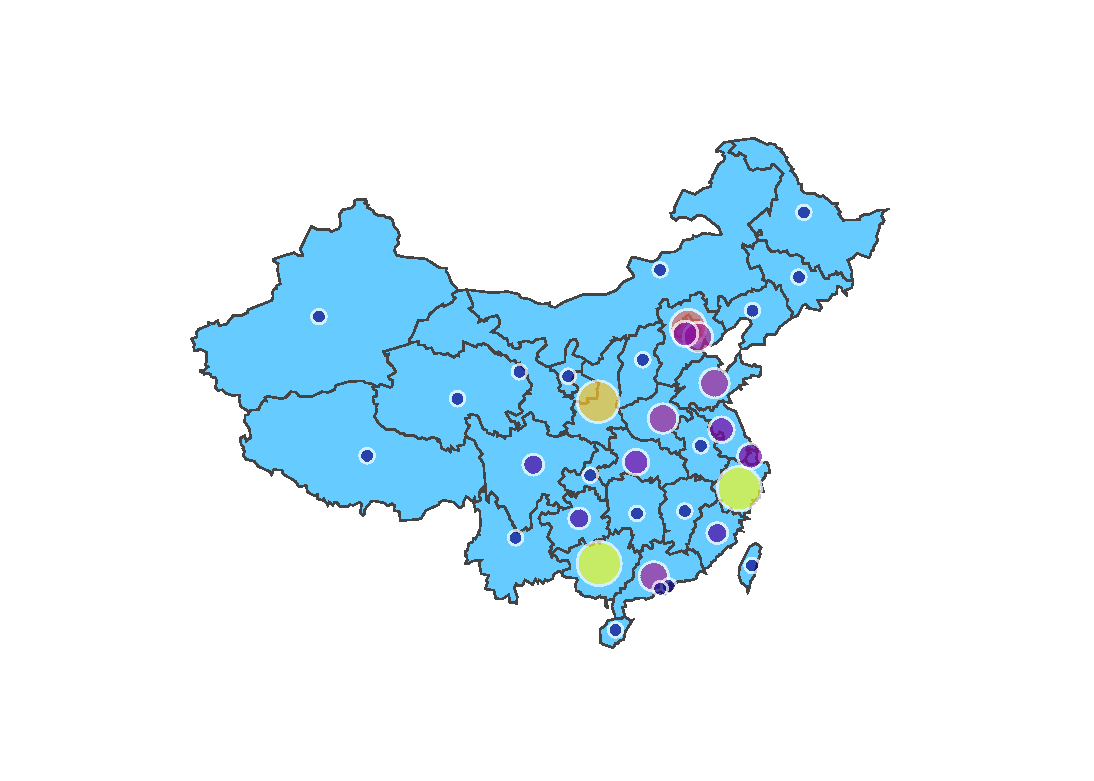
\includegraphics[width=\textwidth]{../figures/covid_rumor_num_choropleth_2}
         \caption{2022-01-08至2022-02-18}
         \label{subfig:covid_rumor_num_choropleth_2}
     \end{subfigure}
    \caption{疫情谣言数量的演化}
    \label{fig:covid_rumor_num_evolution}
\end{figure}

\begin{figure}[!ht]
    \centering
    \begin{subfigure}[b]{0.45\textwidth}
        \centering
        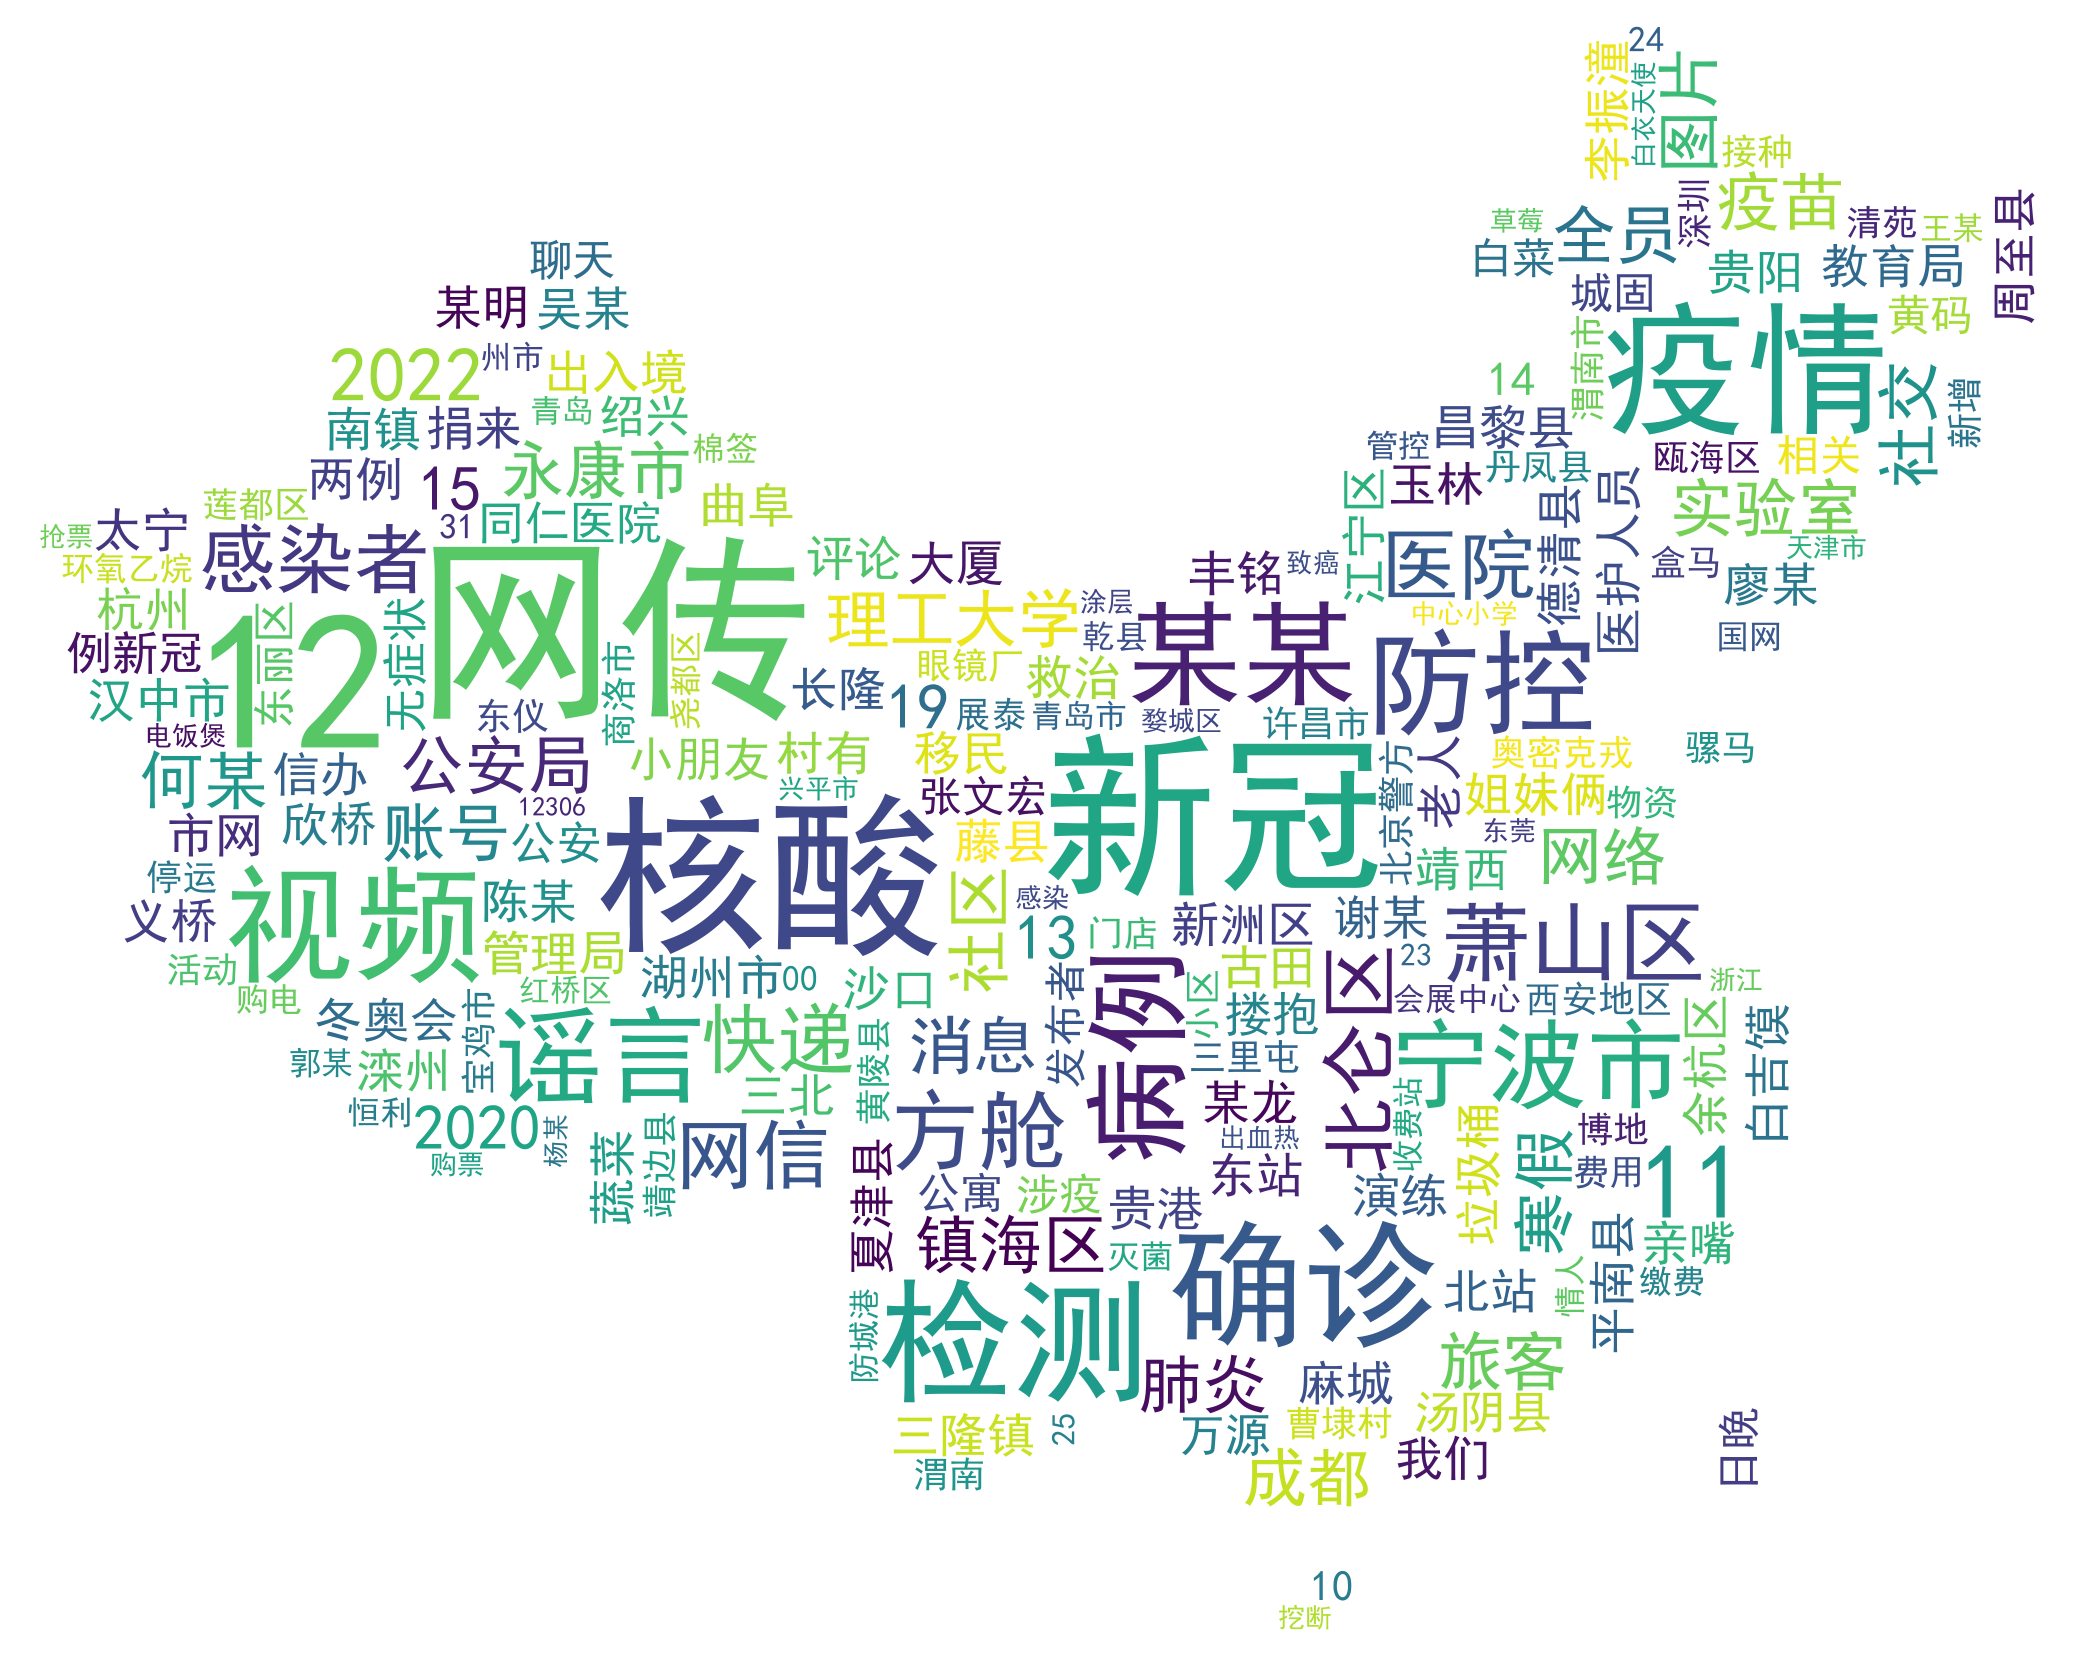
\includegraphics[width=\figwidth]{../figures/wordcloud_covid}
        \caption{疫情谣言}
        \label{subfig:wordcloud_covid}
    \end{subfigure}
    \hfill
    \begin{subfigure}[b]{0.45\textwidth}
        \centering
        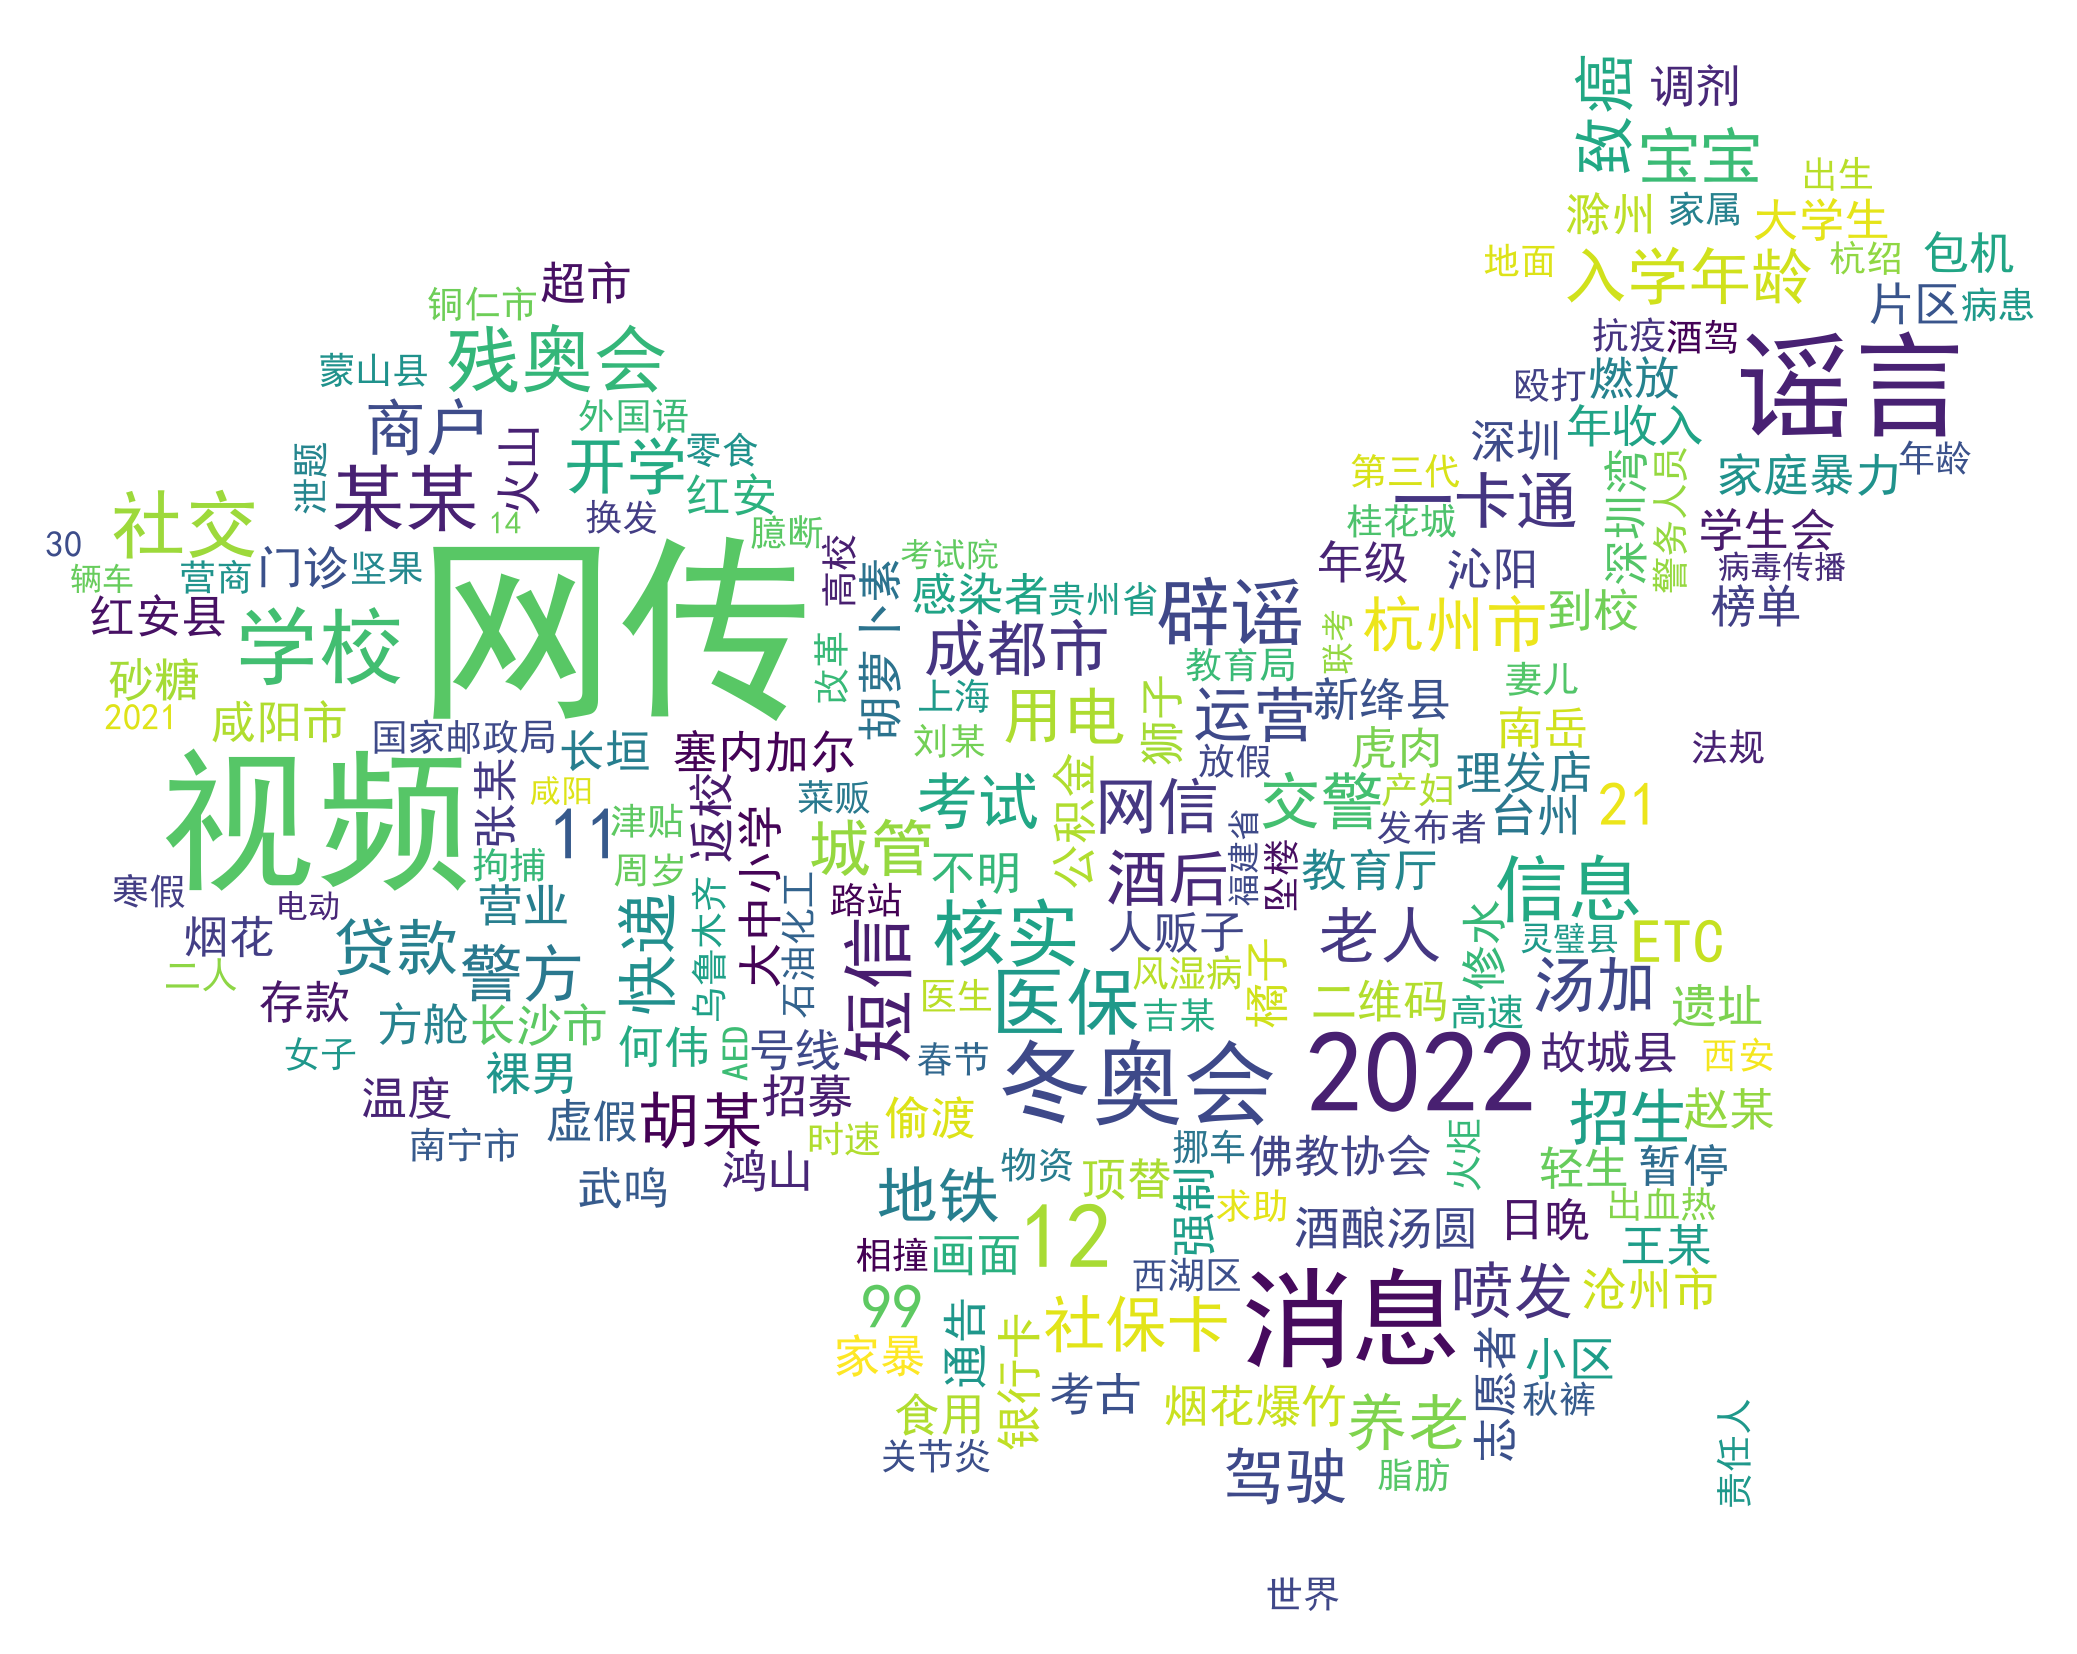
\includegraphics[width=\figwidth]{../figures/wordcloud_nocovid}
        \caption{非疫情谣言}
        \label{subfig:wordcloud_nocovid}
    \end{subfigure}
    \caption{疫情谣言和非疫情谣言的词云}
    \label{fig:wordcloud_covid}
\end{figure}

图~\ref{fig:wordcloud_covid}~展示了疫情谣言和非疫情谣言的词云。从疫情谣言的词云中可以看出,
和疫情有强相关的词语占比很大,值得注意的是,“宁波市”、“萧山区”这些浙江地名占比也很大,说明关于浙江的疫情谣言很多。
非疫情谣言则没有很明显的特征,各种话题都有涉及,值得注意的是“冬奥会”一词占比较大,这和2022年北京冬奥会有所关系。

\section{总结与展望}

在本次研究中,我们首先对谣言数据集进行数据预处理,处理了数据缺失值、重复值,进行了数据类型转换,变量数值变换,分词处理;
之后,我们进行数据可视化的分析,从中我们得到了以下几点结论:
\begin{enumerate}
    \item 谣言数量呈现如下趋势:谣言数量在2021年11月中旬到12月中旬呈现上升趋势;12月中旬到2022年1月中旬保持高位;1月中旬到2月中旬呈现明显下降趋势。谣言数量的地理分布呈现三级分化:西部地区谣言数量很少;华中谣言数量居中,但仍然较少;华北、华南地区谣言数量较多。
    \item 谣言内容中和新冠疫情相关的词语占据了很大的比重,通过LDA方法挖掘5个主题,前3个主题都和疫情强相关,而后2个主题也与疫情相关,但融合了其他的话题。
    \item 数据集中的18位用户可以被分成3个社区,社区1中的用户倾向于浏览有关疫情发展的谣言,社区2中的用户倾向于浏览有关疫情防控的谣言,社区3中的用户倾向于浏览有关疫情之外生活上的谣言。
    \item 疫情相关谣言占谣言的比重很高,达45\%;有关疫情的谣言呈现明显的高峰和低谷,和疫情发展息息相关;疫情的演变是谣言数量的地理分布演变的主要因素;
\end{enumerate}

随着2023年初的逐渐放开,关于疫情的讨论、分析、统计也淡出了人们的视野,虽然现在很多人会遭受“二阳”甚至“三阳”的困扰,但是就舆论而言,疫情已经不是人们关注的焦点。
虽然关于疫情的谣言也有,但不会像数据集所呈现的在2021年底那样绝对数量这么多,占谣言的比重这么高。
分析疫情谣言的传播规律,可以在下个黑天鹅事件到来时,更好地应对谣言的传播,减少谣言对社会的负面影响。

%\appendix
%\section{附录}
%
%\subsection{停用词表} \label{subsec:stopwords}

\end{document}